\documentclass[a4paper,11pt,openany]{kth-mag}
\usepackage[T1]{fontenc}
\usepackage{textcomp}
\usepackage{lmodern}
\usepackage{amsmath}
\usepackage[utf8]{inputenc}
\usepackage[swedish,english]{babel}
\usepackage{csquotes}
\usepackage{csvsimple}
\usepackage{hyperref}
\usepackage{tocloft}
\usepackage{enumitem}
\usepackage[figuresleft]{rotating}

% Default fixed font does not support bold face
\DeclareFixedFont{\ttb}{T1}{txtt}{bx}{n}{12} % for bold
\DeclareFixedFont{\ttm}{T1}{txtt}{m}{n}{12}  % for normal

% Custom colors
\usepackage{color}
\definecolor{deepblue}{rgb}{0,0,0.5}
\definecolor{deepred}{rgb}{0.6,0,0}
\definecolor{deepgreen}{rgb}{0,0.5,0}

\usepackage{listings}
\usepackage[dvipsnames]{xcolor}

\usepackage{fancyvrb}
\fvset{frame=lines,rulecolor=\color{Gray},framesep=1mm,fontfamily=courier,fontsize=\tiny,numbersep=1mm,commandchars=\\\{\}}

% redefine \VerbatimInput
\RecustomVerbatimCommand{\VerbatimInput}{VerbatimInput}%
{
 %
 frame=lines,  % top and bottom rule only
 framesep=2em, % separation between frame and text
 rulecolor=\color{Gray},
 %
 %label=\fbox{\color{Black}data.txt},
 labelposition=topline,
 %
 %commandchars=\|\(\), % escape character and argument delimiters for
                      % commands within the verbatim
 commentchar=*        % comment character
}


% Python style for highlighting
\newcommand\pythonstyle{\lstset{
language=Python,
basicstyle=\ttm,
otherkeywords={self},             % Add keywords here
keywordstyle=\ttb\color{deepblue},
emph={MyClass,__init__},          % Custom highlighting
emphstyle=\ttb\color{deepred},    % Custom highlighting style
stringstyle=\color{deepgreen},
frame=tb,                         % Any extra options here
showstringspaces=false            % 
}}


% Python environment
\lstnewenvironment{python}[1][]
{
\pythonstyle
\lstset{#1}
}
{}

% Python for external files
\newcommand\pythonexternal[2][]{{
\pythonstyle
\lstinputlisting[#1]{#2}}}

% Python for inline
\newcommand\pythoninline[1]{{\pythonstyle\lstinline!#1!}}

\usepackage{modifications}
\usepackage[                    % References
        backend=biber
    ]{biblatex}
    \addbibresource{references.bib}
\usepackage{standalone}
\def\code#1{\texttt{#1}}

\title{Parallelization of dataset transformation with processing order constraints in Python}

\subtitle{Duis autem vel eum iruire dolor in hendrerit in
          vulputate velit esse molestie consequat, vel illum
          dolore eu feugiat null}
\foreigntitle{Lorem ipsum dolor sit amet, sed diam nonummy nibh eui
              mod tincidunt ut laoreet dol}
\author{Dexter Gramfors}
\date{June 2016}
\blurb{Master's Thesis at NADA\\Supervisor: Stefano Markidis\\Examiner: Erwin Laure}
\trita{TRITA xxx yyyy-nn}
\begin{document}
\frontmatter
\pagestyle{empty}
\removepagenumbers
\maketitle
\selectlanguage{english}
\begin{abstract}
    Financial data is often represented with rows of values, contained in a dataset. This data needs to be transformed into a common format in order for
comparison and matching to be made, which can take a long time for larger datasets.
The main goal of this master’s thesis is speeding up these transformations through parallelization using Python multiprocessing.
The datasets in question consist of several rows representing trades, and are transformed into a common format using rules known as filters. In order to devise a
parallelization strategy, the filters were analyzed in order to find ordering constraints, and the Python profiler cProfile was used to find bottlenecks
and potential parallelization points. This analysis resulted in the use of a task-based approach for the implementation, in which the transformation
was divided into an initial sequential pre-processing step, a parallel step where chunks of several trade rows were distributed among workers, and a
sequential post processing step. 

The implementation was tested by transforming four datasets of differing sizes using up to 16 workers, and execution time and memory consumption
was measured. The results for the tiny, small, medium, and large datasets showed a speedup of 0.5, 2.1, 3.8, and 4.81. They also showed linearly increasing
memory consumption for all datasets.  The test transformations were also profiled in order to understand the parallel program’s behaviour for the
different datasets. The experiments gave way to the conclusion that dataset size heavily influences the speedup, partly because of the fact that
the sequential parts become less significant.  In addition, the large memory increase for larger amount of workers is noted as a major downside of
multiprocessing when using caching mechanisms, as data is duplicated instead of shared.

This thesis shows that it is possible to speed up the dataset transformations using chunks of rows as tasks, though the speedup is relatively low.

\end{abstract}
\clearpage
\begin{foreignabstract}{swedish}
    Finansiell data representeras ofta med rader av värden, samlade i en datamängd. Denna data måste transformeras
till ett standardformat för att möjliggöra jämförelser och matchning. Detta kan ta lång tid för stora
datamängder. Huvudmålet för detta examensarbete är att snabba upp dessa transformationer genom parallellisering
med hjälp av Python-modulen multiprocessing. Datamängderna omvandlas med hjälp av regler, kallade filter.
Dessa filter analyserades för att identifiera begränsningar på ordningen i vilken datamänden kan behandlas,
och därigenom finna en parallelliseringsstrategi. Python-profileraren cProfile användes även för att hitta
potentiella parallelliseringspunkter i koden. Denna analys resulterade i användandet av ett ``task''-baserat
tillvägagångssätt, där transformationen delades in i ett sekventiellt pre-processingsteg, ett parallelt steg 
där grupper av rader distribuerades ut bland arbetarprocesser, och ett sekventiellt post-processingsteg.

Implementationen testades genom transformation av fyra datamängder av olika storlekar, med upp till 16 
arbetarprocesser. Resultaten för de fyra datamängderna var en speedup på 0.5, 2.1, 3.8 respektive 4.81.
En linjär ökning i minnesanvändning uppvisades även. Experimenten resulterade i slutsatsen att
datamängdens storlek var en stor faktor i hur mycket speedup som uppvisades, delvis på grund av faktumet
att de sekventiella delarna tar upp en mindre del av programmet. Den stora minnesåtgången noterades som
en nackdel med att använda multiprocessing i kombination med cachning, på grund av duplicerad data.

Detta examensarbete visar att det är möjligt att snabba upp datamängdstransformation genom att använda
radgrupper som tasks, även om en relativt låg speedup uppvisades.

\end{foreignabstract}
\clearpage
\tableofcontents*
\clearpage
\listoffigures
\mainmatter
\chapter*{Definitions}
\addtocontents{toc}{\cftpagenumbersoff{chapter}}
\addcontentsline{toc}{chapter}{Definitions}
\addtocontents{toc}{\cftpagenumberson{chapter}}
\begin{itemize}[label={}, leftmargin=*]
  \item \textbf{IPC} - Interprocess communication.
  \item \textbf{MPI} - Message Passing Interface. Standardized interface for message passing between processes.
  \item \textbf{Embarrassingly parallel} - A problem that is embarrassingly parallel can easily be broken down into components that
    can be run in parallel. %Cite astro? Python hpc?
  \item \textbf{CPU bound} - Calculation where the bottleneck is the time it takes for a processor to execute it.
  \item \textbf{I/O bound} - Calculation where the bottleneck is the time it takes for some input/output call, such as file accesses
    and network operations.
  \item \textbf{Real time} - The total time it takes for a call to finish; ``wall clock'' time.
  \item \textbf{User time} - The time a call takes, excluding system overhead; the time the call spends in user mode.
  \item \textbf{System time} - The time in a call that is consumed by system overhead; the time the call spends in kernel mode.
  \item \textbf{DAG/Directed acyclic graph} A directed graph that contains no directed cycles.
\end{itemize}

\pagestyle{newchap}
\chapter{Introduction}
    In this chapter, an introduction to the parallel computing problem domain and the specific problem of dataset transformation are
described in order to give the reader an initial view of what this thesis entails.

\section{Dataset transformation} \label{dataset_standardization}
In financial applications concerning trading, it is common for customers to upload datasets containing several rows describing trades, which may be in different formats.
One such application is triResolve, an application created in Python and maintained by TriOptima, where this thesis is conducted. 
In triResolve, customers resolve trade disputes in the OTC (Over-The-Counter) derivatives market,
which may arise due to for example differences in valuation methods.
To be able to resolve the trade disputes, customers upload the previously mentioned trade datasets to the service.

The datasets need to be processed in order to transform them into a standard format which makes comparisons between data from different customers possible.
In some cases, the size of the dataset is large enough that this transformation is slow. Out of the possible techniques for optimizing the transformation code,
this thesis will focus on parallelization. Since Python is the language used in triResolve, the parallelization of the existing program will be implemented using
parallel programming tools available in the language. 

When parallelizing a program, the workload is divided among multiple cores of a system, which execute the program in parallel.
For the dataset transformation problem, this means dividing the dataset, conceivably into chunks of rows, and performing the transformation of each of these chunks
on separate cores.

This thesis presents the challenges associated with this parallelization problem, and how to solve them.

%In some cases, the size of the dataset is large enough that this transformation is slow, and could conceivably be sped up through
%the use of parallelization. The sizes are aptly measured in number of rows, and range between 2 rows to about 1490000 rows. The time
%it takes to process the datasets range between 0.06 seconds and 15200 seconds 2 (4.2 hours).

%\subsection{Transformation with constraints}
The datasets are associated with a file format. The format specifies a set of rules, known as filters, which at times enforce
implicit constraints on the processing order in the file when performing the transformation. This thesis aims to identify these
constraints, which may affect how parallelizable a dataset is, and find a suitable parallelization strategy. Another aim is to identify the impact dataset size has on
any potential speedup. In addition, how using the Python \code{multiprocessing} module and its process-over-thread with message passing
approach affects implementation and performance will be investigated.

\section{Parallel computing}
In this thesis, a task-based approach is used to parallelize the dataset transformation \cite{chow_2015_pipeline_ppiaote}. A task is a single unit of computation, often represented as a function
and run on different threads or processes. Tasks are executed by the operating system's scheduler, and can be executed on different cores. When tasks are scheduled
on different cores, they are able to run at the same time, resulting in parallelism and possible speedup of a program. If there are more tasks than cores, the tasks
are scheduled using time-slicing, where tasks share cores.

\section{Hardware}
The parallelization in this thesis is conducted on a shared memory computer. In this setup, several computing units (cores) share one memory. Examples of
shared memory systems are common laptops and workstations.

%reduce the possible benefits of parallelization as they enforce
%inherently serial parts of the transformation program.  Since the size of the datasets as well as the type and number of their
%associated filters varies, it is plausible that the benefits of parallelization will differ significantly between different datasets.
%An overhead is associated with creating new threads or processes.  This overhead is increased in Python as the data shared between processes needs to serialized.
%Therefore, it is possible that parallelization of datasets will result in slower execution in some cases. Consequently, it is
%interesting to find the combinations of dataset sizes, as well as their filters, that result in beneficial parallelization, and which do not.
%Additionally, the complex nature of the system makes the implementation of the parallelization an interesting problem.

%\section{Parallel computing}
%The subject of parallel computing is one that has become highly relevant in recent years.
%Moore's law, the observed pattern that the number of transistors in a dense integrated circuit doubles approximately every two
%years \cite{moore_1998_cramming_cmcoic},
%has lost its relevance. The increased processor clock speed that the doubling in processors implies is no longer present because of
%overheating issues \cite[p. 1]{herlihy_2012_art_taomprr}. Because of this, manufacturers of processors now have
%largely turned to \emph{multicore} processors. In a multicore architecture, several cores which work as individual processors execute
%code simultaneously. Using this type of architecture to work on a single task to increase performance is known as \emph{parallelism}.

%Efforts to exploit parallelism automatically from a program have been made; however, the benefits of these have reached their
%limit \cite[p. 7-12]{mccool_2012_structured_spppfec}. In order to fully utilize the increase in performance that multicore
%architectures promise, programmers today must instead turn to explicit parallel programming.

%Python is one of world's most popular programming languages \cite{krill_2015_python_psnhilp}. It is used extensively both at schools and
%in the industry, and its benefits include expressiveness, portability, and the fact that it is easy to learn. Python has support for
%parallel programming, although it has caveats and overheads associated with a concurrency-hampering mechanism called the
%\emph{Global Interpreter Lock} \cite{beazley_150745UTC_introduction_aitpc}.

%This thesis concerns a combination of the areas mentioned above: parallel computing using Python.

%\section{Dataset transfromation} \label{trioptima}
%The thesis is conducted at TriOptima, a company that provides different services for the OTC derivatives market.
%In one of TriOptima's services, customers upload datasets representing trades.
%OTC derivatives concern trading directly between two parties, and the customers include large banks. TriOptima’s services
%include portfolio compression, reconciliation, dispute resolution, and risk management. The services deal with substantial
%amounts of data, and face challenges such as high security demands, availability requirements, and speed optimization
%for data transformations and risk calculations. In their reconciliation and dispute resolution service,

\section{Motivation}
The motivation of this thesis is to answer the following questions.

\emph{Given the size of a dataset and its set of filters, is it possible to determine 
if parallelization of the data transformation using Python will be beneficial or not?}

The thesis question gives rise to the following subquestions:
\begin{itemize}
    \item What is the best approach for parallelizing code in Python in order to minimize data races and maintain performance?
    \item How should the parallel performance be measured?
    \item What kind of data dependencies exist and how do they affect parallelization?
    \item What kind of overhead does parallelization introduce?
\end{itemize}

\section{Objectives}
The objectives of this thesis are to:
\begin{itemize}
    \item Analyze parallelizability of dataset file formats.
    \item Use a Python profiler to analyze \code{multiprocessing} performance for dataset transformation.
    \item Implement a working parallelization of the dataset transformation program, for the applicable datasets.
    \item Evaluate the parallel performance of transformation of different datasets by measuring execution time, speedup, and memory consumption.
\end{itemize}
%The objective of this thesis is to answer the questions stated above using a literature study and by implementing a working parallelization
%of the existing dataset processing program, subsequently analysing transformations of several datasets in order to draw conclusions about performance.

\section{Contribution}
This thesis focuses on parallelization analysis of a file format rather than the more conventional method of analyzing source code. Additionally,
it shows how Python can be effectively used for parallelization in a complex system not built for parallelization from the start. The fact that
the parallelized system relies on database operations and, consequently, I/O is another aspect of the thesis that may interest other researchers
in the field of parallel programming. Similar projects can use the conclusions of this thesis as a foundation when creating a parallelization strategy.

\chapter{Background}
    Purpose of chapter, TODO

\section{Definitions}
\begin{itemize}
  \item \emph{IPC} Interprocess communication.
  \item \emph{MPI} Message Passing Interface. Standardized interface for message passing between processes.
  \item \emph{Embarrassingly parallel} A problem that is embarrassingly parallel can easily be broken down into components that
    can be run in parallel. %Cite astro?
  \item \emph{Real time} The total time it takes for a call to finish.
  \item \emph{User time} The time a call takes, excluding system overhead; the time the call spends in user mode.
  \item \emph{System time} The time in a call that is consumed by system overhead; the time the call spends in kernel mode.
\end{itemize}

\section{Multicore architecture} %Find a better name?
\subsection{Processes vs threads}
while both threads and processes represent contexts in which a program is run, they have a few differences. A thread is run inside
a process, and the threads within the process share memory and state with each other and the parent
process \cite{singh_2013_parallel_padpwprfmm}. Individual processes do not share memory with each other, and any
communication between processes must be done with message passing rather than with shared memory. Consequently, communication
between threads is generally faster than between processes.
Typically, different threads can be scheduled on different cores, which is also true for different processes. %Fixa citation

\subsection{Scheduling}
Threads and processes are scheduled by the operating system, and the exact mechanism for choosing what to schedule when differs
between platforms and implementations \cite[p. 472]{herlihy_2012_art_taomprr}. Scheduling may imply running truly parallel
on different cores, or on the same core using time-slicing. Threads and processes may be descheduled from running temporarily for several
reasons, including issuing a time-consuming memory request.

\subsection{Multicore communication and caching}
Multiple processors communicate with each other through a bus or a network \cite[p. 472-476]{herlihy_2012_art_taomprr}. Since the
means of communication between the processes is a finite resource, too much traffic may result in delays. The processors typically
have their own cache. In order to avoid unnecessary reads from the slower main memory, processors may read from another processor
that has the requested data cached. In a process called \emph{cache coherence}, shared cached values are kept up to date using one
of several protocols. The effect that these different means of communication between processors has on performance in
multiprocessor programs should not be ignored.

\subsection{Data parallelism}
Data parallelism denotes code where the parallelism comes from decomposing the data and running it with the same piece of code
across several processors or computers \cite{singh_2013_parallel_padpwprfmm}. It allows scalability as number of cores and problem
sizes increase, since more parallelism can be exploited for larger data sets \cite[p. 24]{mccool_2012_structured_spppfec}.

\subsection{Task parallelism}
\section{Performance models for parallel speedup}
\subsection{Amdahl's law}
\subsection{Expanding Amdahl's law}
\subsection{Work-span model}
\section{Python performance and parallel capabilities}
\subsection{Performance}
\subsection{The GIL, Global Interpreter Lock}
\subsection{Threading}
\subsection{Multiprocessing}

\section{Related work}
\subsection{Efficient parallelization of path planning workload on single-chip shared-memory multicores}
Ahmad et al. \cite{ahmad_2015_efficient_epoppwossm} parallelize path planning algorithms such as Dijkstra's algorithm using C/C++ and
Python in order to compare the results and evaluate each language's suitability for parallel computing. For the Python implementation,
both the \code{multiprocessing} and \code{threading} packages are used. The authors identify Python as the preferable choice 
in application development, due to its safe nature in comparison to C and C++. The implementation using the \code{threading}
module resulted in no speedup over the sequential implementation. Parallelization using the \code{multithreading} module resulted
in a speedup of 2.5x for sparse graphs, and a speedup of 6.5x for dense graphs. The overhead introduced by the interpreted nature
of Python, as well as the extra costs associated with Python multiprocessing, was evident as the C/C++ implementations showed both
better performance and better scalability. The slowdowns for sparse graph of Python compared to C/C++ ranged between
20x to 700x depending on the graphs.
However, the authors note that the parallel Python implementation exhibits scalability in comparison to its sequential implementation.

The experiments were conducted on a machine with 4 cores with 2-way hyperthreading.


\subsection{Harnessing multicores: Strategies and implementations in ATLAS}
Binet et al. \cite{binet_2010_harnessing_hmsaiia} present a case study where parts of the ATLAS software used in
LHC (Large Hadron Collider) experiments are parallelized. Because of the complexity and sensitivity of the system,
one of the goals of the study is to minimize the code changes when implementing the parallelization. The authors highlight several
benefits of using multiple processes with IPC (interprocess communication) instead of traditional multithreading, including ease of 
implementation, explicit data sharing, and easier error recovery. The Python \code{multiprocessing} module was used to parallelize
the program, and the authors emphasize the decreased burden thanks to not having to implement explicit IPC and synchronization.
Finding the parts of the program that is embarrassingly parallel (DEFINE THIS) and parallelizing these is
identified as the preferred approach in order to avoid an undesirably large increase in complexity while
still producing a significant performance boost.

The parallel implementation was tested by measuring the user and real time (DEFINE THESE) for different numbers of processes.
These measurements show a clear increase in user time because of additional overhead, but also a steady decrease in real time.

\subsection{On the Performance of the Python Programming Language for Serial and Parallel Scientific Computations}
Cai et al. \cite{cai_2005_performance_otpotpplfsapsc} note that Python is suitable for scientific programming thanks to its richness and
power, as well as its interfacing capabilities with legacy software written in other languages. Among other experiments on Python
efficiency in scientific computing, its parallel capabilities are investigated. The Python MPI (DEFINE) package \code{Pypar} is used for
the parallelization, using typical MPI operations such as send and receive. The calculations, such as wave simulations, 
are made with the help of the \code{numpy} package for increased efficiency. The authors conclude that while communication 
introduces overhead, Python is sufficiently efficient for scientific parallel computing.

\subsection{Parallel astronomical data processing with Python: Recipes for multicore machines}
Singh et al. \cite{singh_2013_parallel_padpwprfmm} present Python as a fitting language for parallel computing, and use the
\code{multiprocessing} module as well as the standalone \code{Parallel Python} package in their experiments. Because of the
communication overhead in Python, the study focuses on embarrassingly parallel problems where little communication is needed.
Different means of parallelization are
compared: the Pool/Map approach, the Process Queue approach, and the Parallel Python approach. %TODO: Maybe define the approaches?
The results in general show significant time savings even though the approaches taken are relatively straightforward.
The best performance is achieved when the number of processes is equal to the number of physical cores on the computer.
The Process/Queue is shown to perform better than both Pool/Map and parallel Python. This comes at the cost of a slightly less
straightforward implementation. The impact of load balancing and chunk size is also discussed, with the conclusion that work load
should be evenly distributed among cores as computation is limited by the core that takes the longest to finish.

\subsection{Parallel optimal choropleth map classification in PySAL}
Rey et al. \cite{rey_2013_parallel_pocmcip} compare \code{multiprocessing} and \code{Parallel Python} with the GPU-based parallel
module \code{PyOpenCI} when attempting to parallelize portions of the spatial analysis library PySAL. In particular, different
versions of the Fisher-Jenks algorithm for classification are compared. For the smallest sample sizes, the overhead of the
different parallel implementations produce slower code, but as the sample sizes grow larger the speedup grow relatively quickly.
For the largest of the sample sizes, the speedup curve generally flattens out; the authors state this as counter-intuitive and
express an interest in investigating this further. In general, the CPU-based modules \code{multiprocessing} and \code{Parallel Python}
perform better than the GPU-based PyOpenCI. The \code{multiprocessing} module produced similar or better results than the
\code{Parallel Python} module.
While the parallel versions of the algorithm perform better, the bigger implementation effort associated with it is noted.

\subsection{PEP 0371}
In their proposal for the inclusion of the multiprocessing module into the Python standard library,
Noller and Oudkerk \cite{noller_pep_p0} include several benchmarks where the multiprocessing module's performance is compare to
that of the threading module. They emphasize the fact that the benchmarks are not as applicable on platforms with slow forking
time. The benchmarks show that while of course slower than sequential execution, multiprocessing performs better than
threading when just spawning workers and executing an empty function. For the CPU-bound task of computing Fibonacci numbers,
multiprocessing shows significantly better result than threading (which is in fact slower than sequential code). For I/O bound
calculations, which is an application considered suitable for the threading module, the multiprocessing module is still shown to have
the best performance when 4 or more workers are used.

The benchmarks where performed using the following hardware:
\begin{itemize}
  \item 4 Core Intel Xeon CPU @ 3.00GHz
  \item 16 GB of RAM
  \item Python 2.5.2 compiled on Gentoo Linux (kernel 2.6.18.6)
  \item pyProcessing 0.52
\end{itemize}

\subsection{Three Unique Implementations of Processes for PyCSP}
Friborg et al. \cite{friborg_2009_three_tuiopfp} explore the use of processes, threads and greenlets in their process abstraction
library PyCSP. The authors observe the clear performance benefits of using multiprocessing over threads due to the circumvention of the GIL
that the multiprocessing module allows. Greenlets are user-level threads that execute in the same thread and are unable to utilize
several cores. On Microsoft Windows, where the fork() system call is not available, the process creation is observed as
significantly slower than on UNIX-based platforms. While serialization and communication has a negative impact on performance when
using multiprocessing, the authors state that this produces the positive side-effect of processes not being able to
modify data received from other processes.

\subsection{Summary of related work}
Common themes and conclusions in the related work presented above include.

\begin{itemize}
  \item Python is a suitable language for parallel programming.
  \item The multiprocessing module is successful in circumventing the GIL often shows the same or better performance than other
    methods, even for I/O bound programs.
  \item The overhead that IPC introduces when creating parallel Python programs makes it imperative to minimize communication and
    synchronization. Consequently, embarrassingly parallel programs are preferable when using Python.
  \item For existing larger systems, extensive parallelization may produce undesired complexity.
\end{itemize}

\chapter{Related work}
    In this section, work related to that of this thesis is summarized and discussed, in order to utilize conclusions made by
others when deciding upon the method to use, and also to highlight differences between earlier works and this thesis.
\section{Parallelization of algorithms using python}

Ahmad et al. \cite{ahmad_2015_efficient_epoppwossm} parallelize path planning algorithms such as Dijkstra's algorithm using C/C++ and
Python in order to compare the results and evaluate each language's suitability for parallel computing. For the Python implementation,
both the \code{multiprocessing} and \code{threading} packages are used. The authors identify Python as the preferable choice 
in application development, due to its safe nature in comparison to C and C++. The implementation using the \code{threading}
module resulted in no speedup over the sequential implementation. Parallelization using the \code{multithreading} module resulted
in a speedup of 2.5x for sparse graphs, and a speedup of 6.5x for dense graphs. The overhead introduced by the interpreted nature
of Python, as well as the extra costs associated with Python multiprocessing, was evident as the C/C++ implementations showed both
better performance and better scalability. The slowdowns for sparse graph of Python compared to C/C++ ranged between
20x to 700x depending on the graphs.
However, the authors note that the parallel Python implementation exhibits scalability in comparison to its sequential implementation.
The experiments were conducted on a machine with 4 cores with 2-way hyperthreading.

Cai et al. \cite{cai_2005_performance_otpotpplfsapsc} note that Python is suitable for scientific programming thanks to its richness and
power, as well as its interfacing capabilities with legacy software written in other languages. Among other experiments on Python
efficiency in scientific computing, its parallel capabilities are investigated. The Python MPI package \code{Pypar} is used for
the parallelization, using typical MPI operations such as send and receive. The calculations, such as wave simulations, 
are made with the help of the \code{numpy} package for increased efficiency. The authors conclude that while communication 
introduces overhead, Python is sufficiently efficient for scientific parallel computing.

Singh et al. \cite{singh_2013_parallel_padpwprfmm} present Python as a fitting language for parallel computing, and use the
\code{multiprocessing} module as well as the standalone \code{Parallel Python} package in their experiments. Because of the
communication overhead in Python, the study focuses on embarrassingly parallel problems where little communication is needed.
Different means of parallelization are
compared: the Pool/Map approach, the Process/Queue approach, and the Parallel Python approach. 
In the Pool/Map approach, the simple functions of \code{multiprocessing.Pool} are used to specify a number of processes, a data
set, and the function to be executed with each element in the dataset as a parameter. In the Process/Queue approach, a
\code{multiprocessing.Queue} is spawned and filled with chunks of data. Several \code{multiprocessing.Process} objects are then
spawned, which all share the queue and get data to operate on from it while it is not empty. Another shared queue is used for
collecting the results. In the Parallel Python approach, the \code{Parallel Python} abstraction \emph{job server}
is used to submit tasks for each data chunk. The tasks are automatically executed in parallel by the job server, and the results
are collected when they have finished.  The results in general show significant time savings even though the approaches taken are relatively straightforward.
The best performance is achieved when the number of processes is equal to the number of physical cores on the computer.
The Process/Queue is shown to perform better than both Pool/Map and parallel Python. This comes at the cost of a slightly less
straightforward implementation. The impact of load balancing and chunk size is also discussed, with the conclusion that work load
should be evenly distributed among cores as computation is limited by the core that takes the longest to finish.

Rey et al. \cite{rey_2013_parallel_pocmcip} compare \code{multiprocessing} and \code{Parallel Python} with the GPU-based parallel
module \code{PyOpenCI} when attempting to parallelize portions of the spatial analysis library PySAL. In particular, different
versions of the Fisher-Jenks algorithm for classification are compared. For the smallest sample sizes, the overhead of the
different parallel implementations produce slower code, but as the sample sizes grow larger the speedup grows relatively quickly.
For the largest of the sample sizes, the speedup curve generally flattens out; the authors state this as counter-intuitive and
express an interest in investigating this further. In general, the CPU-based modules \code{multiprocessing} and \code{Parallel Python}
perform better than the GPU-based PyOpenCI. The \code{multiprocessing} module produced similar or better results than the
\code{Parallel Python} module.
While the parallel versions of the algorithm perform better, the bigger implementation effort associated with it is noted.

In the work above, the code that is parallelized is strictly CPU bound. This differs from this thesis, as a portion of the
to be parallelized program is I/O bound due to database interactions. Another difference is the fact that
the parallelization analysis conducted in this thesis is mainly done on the file format level rather than at program level, like the work above.
However, the works highlight aspects of parallelization using Python that are useful in achieving the thesis objective.
These include parallelization patterns, descriptions of overhead associated with parallel programming in Python, and comparisons
between different Python modules for parallelization.

\section{Python I/O performance and general parallel benchmarking}
In their proposal for the inclusion of the \code{multiprocessing} module into the Python standard library,
Noller and Oudkerk \cite{noller_pep_p0} include several benchmarks where the \code{multiprocessing} module's performance is
compared to that of the \code{threading} module. They emphasize the fact that the benchmarks are not as applicable on platforms with slow forking
time. The benchmarks show that while naturally slower than sequential execution, \code{multiprocessing} performs better than
\code{threading} when simply spawning workers and executing an empty function. For the CPU-bound task of computing Fibonacci numbers,
\code{multiprocessing} shows significantly better result than \code{threading} (which is in fact slower than sequential code). For I/O bound
calculations, which is an application considered suitable for the \code{threading} module, the \code{multiprocessing} module is still shown to have
the best performance when 4 or more workers are used.

While this work is a relatively straightforward benchmark under ideal conditions, the fact that \code{multiprocessing} shows better performance than \code{threading}
for both CPU bound and I/O bound computations contributed to the decision to use \code{multiprocessing} in this thesis.

\section{Comparisons of process abstractions}
Friborg et al. \cite{friborg_2009_three_tuiopfp} explore the use of processes, threads and greenlets in their process abstraction
library PyCSP. The authors observe the clear performance benefits of using multiprocessing over threads due to the circumvention of the GIL
that the \code{multiprocessing} module allows. Greenlets are user-level threads that execute in the same thread and are unable to utilize
several cores. On Microsoft Windows, where the fork() system call is not available, the process creation is observed as
significantly slower than on UNIX-based platforms. While serialization and communication has a negative impact on performance when
using \code{multiprocessing}, the authors state that this produces the positive side-effect of processes not being able to
modify data received from other processes.

The work above focuses on process abstractions in a library, but comes to conclusions that are helpful in this thesis; \code{multiprocessing}
has performance benefits over the other alternatives, and also introduces safety to a system thanks to less modification of data sent between
processes.

\section{Parallelization in complex systems using Python}
Binet et al. \cite{binet_2010_harnessing_hmsaiia} present a case study where parts of the ATLAS software used in
LHC (Large Hadron Collider) experiments are parallelized. Because of the complexity and sensitivity of the system,
one of the goals of the study is to minimize the code changes when implementing the parallelization. The authors highlight several
benefits of using multiple processes with IPC instead of traditional multithreading, including ease of 
implementation, explicit data sharing, and easier error recovery. The Python \code{multiprocessing} module was used to parallelize
the program, and the authors emphasize the decreased burden resulting from not having to implement explicit IPC and synchronization.
Finding the parts of the program that are embarrassingly parallel and parallelizing these is
identified as the preferred approach in order to avoid an undesirably large increase in complexity while
still producing a significant performance boost. The parallel implementation was tested by measuring the user and real time for different numbers of processes.
These measurements show a clear increase in user time because of additional overhead, but also a steady decrease in real time.

Implementing parallelization of a component of a large system without introducing excessive complexity is a goal of this thesis, similar to the work above.
The above approach to parallelization, identifying embarrassingly parallel parts of the system and focusing on these, were used in this thesis. Again, 
this thesis differs from the above by having an I/O bound portion and by analysing a file format for parallelizability.

\section{Summary of related work}
Common themes and conclusions in the related work presented above include:

\begin{itemize}
  \item Python is a suitable language for parallel programming.
  \item The \code{multiprocessing} module is successful in circumventing the GIL and consistently shows the same or better performance than other
    methods, even for I/O bound programs.
  \item The overhead that IPC introduces when creating parallel Python programs makes it imperative to minimize communication and
    synchronization. Consequently, embarrassingly parallel programs are preferable when using Python for parallelization.
  \item For existing larger systems, extensive parallelization may produce undesired complexity.
\end{itemize}
 \label{related_work}
\chapter{Dataset Transformation}
    \section{Technology}
In this section, technologies used in the transformation program that will be mentioned throughout this chapter are briefly described.

\subsection{Django}
Django is a Python web development framework \cite{holovaty_chapter_c1itd}. It implements a version of the MVC (Model-View-Controller) pattern, which decouples request routing, data access, and
presentation. Django's model layer allows the programmer to retrieve and modify entities in an SQL database through Python code, without writing SQL.

\subsection{MySQL}
MySQL is an open source relational database system \cite{what_wim}. It is used by TriOptima as the database backend for Django.

\subsection{Cassandra}
Cassandra is a column-oriented \textit{NoSQL} database \cite[p. 1-9]{mishra_2014_beginning_bacd}. It features dynamic schemas, meaning that columns can be added dynamically to a schema as needed, and that
the number of columns may vary from row to row. Cassandra is designed to have no single point of failure, and uses a number of nodes in a peer-to-peer structure. This design is
employed in order to ensure high availability, with data replicated across the nodes.

\section{Performance analysis tools}
\subsection{cProfile}
A Python profiler with a relatively low overhead, which can be invoked both directly in a Python program and form the command line \cite{26_2tppp2d}.
An example of the way cProfile is used in this thesis can be found in figure \ref{fig:profiler_example}.

\begin{figure}[ht]
  \centering
  \pythonexternal{code_examples/profile_example.py}
  \caption{\code{cProfile} usage example.}
  \label{fig:profiler_example}
\end{figure}

\subsection{resource}
\code{resource} is a Python module used for measuring resources used by a Python program \cite{36_3rruip2d}. It can be used for finding the user time, system time,
and the maximum memory used by the process.

\section{Trade files and datasets}
As mentioned briefly in section \ref{trioptima}, users of the triResolve service upload \textit{trade files}, which contain one or several datasets with
rows of trade data such as party id, counterparty id, trade id, notional, and so on. An example of a trade dataset (with some columns omitted) can be seen in figure
\ref{fig:data_set_example}.

\begin{figure}[ht]
\centering
\resizebox{\linewidth}{!}{%
\begin{tabular}{|c|c|c|p{3cm}|c|c|}%
  \hline
  \bfseries Party ID & \bfseries CP ID & \bfseries Trade ID & \bfseries Product class & \bfseries Trade curr & \bfseries Notional
  \csvreader[respect all,head to column names]{figures/EFET.csv}{PARTY_ID=\pid, CP_ID=\cpid, TRADE_ID=\tid, PRODUCT_CLASS=\pcls, TRADE_CURR=\tc, NOTIONAL=\notional}
  {\\\hline \pid & \cpid & \tid & \pcls & \tc & \notional}
  \\ \hline
\end{tabular}}
  %\centering
\caption[Example of trade dataset]{A simplified example of a trade dataset uploaded by the users of triResolve.}
  \label{fig:data_set_example}
\end{figure}

\section{File formats}
Different customers may have different ways of formatting their datasets, with different names for headers, varying column orders, extra fields,
and special rules. In order to convert these into a standard format that make it possible to use the files in the same contexts, a file format specifying
how the dataset in question should be processed is used. The format contains a set of \textit{filters} which should be applied to each row of the dataset.
The different filter configurations may affect how parallelizable the processing of the dataset is.

\section{Verification results}
The result of the dataset processing is called a \textit{verification result}\footnote{The verification results are not to be confused with the results of this thesis. They are part of the problem this thesis aims to solve.}, and consists of one row per trade, with correctly modified values, in a Cassandra schema.
In addition, a row in the MySQL database consisting of metadata relating to the result as a whole is created. This metadata includes result owner, number of rows, time metrics, and so on.

\section{Transformation with constraints}
\subsection{Filters}
All filters used to transform a dataset into a verification result are outlined below.

\begin{itemize}
\item \textbf{Header detection} --
There may be a number of initial lines in the dataset which do not contain the header (which specifies the column names). The header detection filter checks if a row is the header,
and if it is it saves the column names and corresponding indices for use in subsequent rows. If the row is not the header or the header has already been detected
(for example if another header row is encountered in the middle of the dataset), this filter terminates without any effect and the rest of the filters are applied.
This filter is included in all file formats.

\item \textbf{Mapping} --
Maps a value from a column in the dataset to a specified output column in the verification result. There is usually a mapping for each of the columns in the input
dataset, and the Mapping filter is therefore one of the most common filters. The mappings may have small extra tuning attached to them, such as specifying a date
format or extracting only part of the text using regex. One of these extra tunings is attached to the trade id column, and is called \textit{Make unique}.
This tuning keeps track of all trade id:s that have been encountered so far, and, if it finds a duplicate, adds a suffix to it in order to ensure that all trade id:s are unique.

\item \textbf{Dataset translation} --
A dataset translation is similar to a mapping, but uses specified columns in an external dataset to map input columns to output columns.

\item \textbf{Dataset information} --
Extracts information about the dataset, such as the name or owner.

\item \textbf{Tradefile information} --
Similar to the dataset information filter, except that it extracts information about the trade file that contains the dataset.

\item \textbf{Null translation} --
In some datasets, other values than \code{NULL} are used to convey the absence of a value. This filter allows the user to specify which other values
should be interpreted as \code{NULL}.

\item \textbf{Relation currency} --
If the currency that is supposed to be used in a relation (a party and a counterparty) is stored in the database and should be mapped to an output column, this
filter retrieves this information.

\item \textbf{Global variable} --
A global variable filter writes a value to a variable that is accessible by subsequent filters on the same row, and by all filters on the rest of the rows in the data
set. A global variable can be written several times throughout the processing of a dataset.

\item \textbf{State variable} --
A state variable is similar to a global variable, but is always written to before all other processing of the dataset begins.

\item \textbf{Temporary variable} --
Similar to the other variables, except for the fact that it is only accessible during processing of the row where it was written. When the 
processing of the row is finished, the variable is cleared.

\item \textbf{Conditional block} --
A conditional block works like the programming construct \code{if}. It performs a specified filter (which may also be a conditional block) only if a certain
condition is fulfilled. Most commonly, the condition takes the form '\code{field = value}', but may also involve more complex expressions in the form of a
subset of Python.

\item \textbf{Logger} --
A logger filter simply logs a given value. Can for instance be used when a user wants to know whenever a conditional block has been entered.

\item \textbf{Skip row} --
Ignores the current row when processing. Usually used in a conditional block.

\item \textbf{Stop processing} --
Stops processing the dataset, ignoring all subsequent rows. Can be used as a subfilter in the Conditional block filter when the footer of the dataset
contains information that should not be interpreted as a trade.

\item \textbf{Third party automapper} --
When a customer has uploaded a trade file on behalf of another customer, this filter extracts the information needed to make sure that the data is loaded
for the correct customer.

\item \textbf{Set value} --
Simply sets the value of the output column to the value that is entered.

\item \textbf{RegExp extract} --
Extracts text from a column using regex, and writes matching groups to other columns.

\item \textbf{RegExp replace} --
Replaces column text matching some regex with a specified value.

\end{itemize}

An example of how filter application and dataset row transformation work can be found in figure \ref{fig:filter_diagram}.

\begin{figure}[ht]
  \centering
  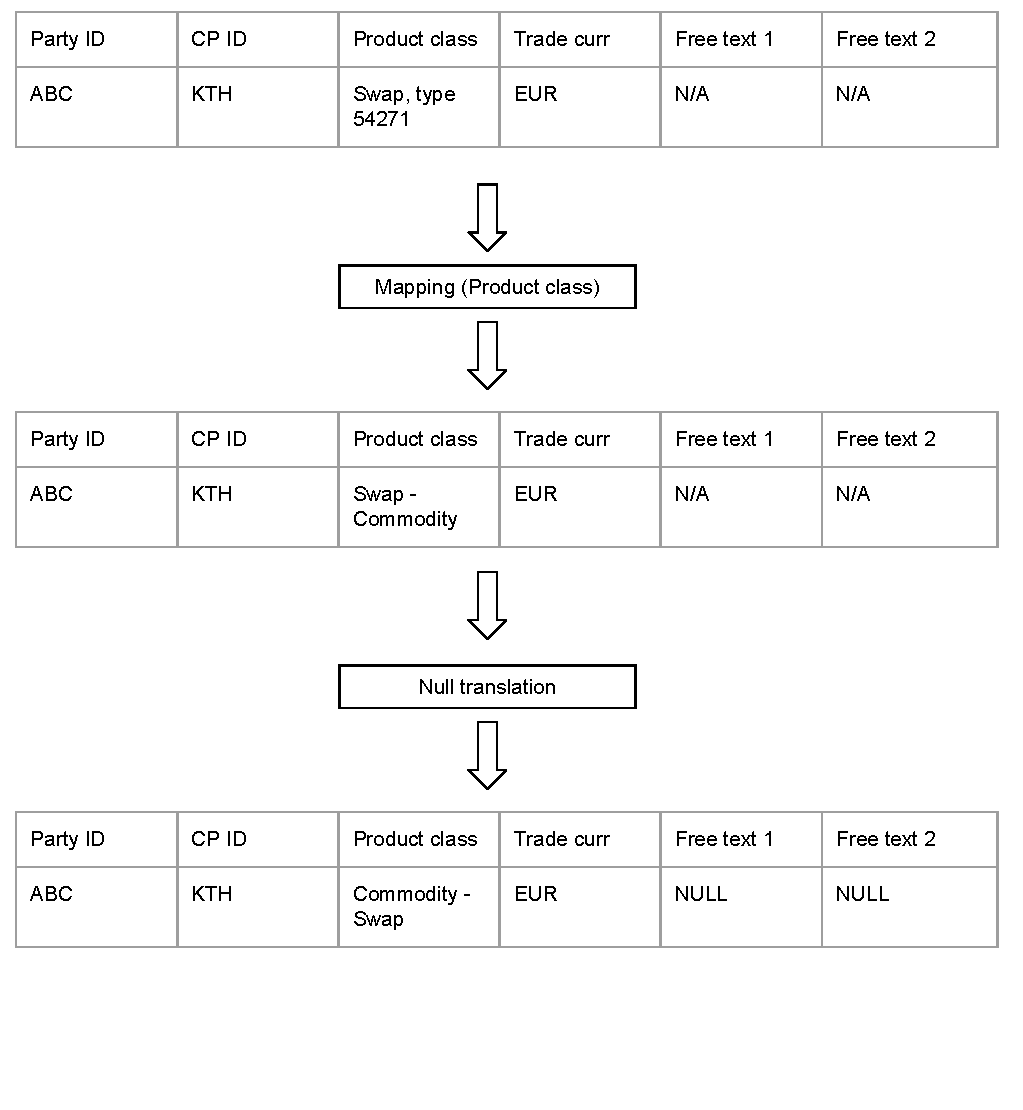
\includegraphics[width=120mm]{figures/filter_diagram.pdf}
  \caption[Filter application example.]{A simplified example of how filter application and dataset transformation work. The mapping filter for the
  product class column is applied, transforming ``Swap, type 54271'' to the standardized ``Swap - Commodity ''. In the file format used for this example,
  ``N/A'' is used to denote the absence of a value, making the null translation filter translate all columns containing ``N/A'' to ``NULL''.}
  \label{fig:filter_diagram}
\end{figure}

\section{Program overview}
The general flow of the original, sequential, dataset processing program is the following:
\\\\
The unprocessed dataset has the rows stored in a Cassandra database, and some metadata and methods stored in a Django object backed by a MySQL database.
The file format corresponding to the dataset is looked up, and all of the filters it contains are added to a pipeline that will process the dataset.
An empty verification result is then created in both Cassandra and MySQL, containing the row data and result metadata with metrics, respectively.
The metrics include processing time, number of trades, timestamp, and similar data. The rows in the dataset are then processed one by one,
applying all filters to each row. As soon as a row has finished processing, it is written to the verification result in Cassandra.
During this process, the row mappings used in the \textit{Mapping} filter are fetched from the MySQL database, resulting in some
I/O waiting time. To mitigate this, the mappings are cached in memory for faster access. After the processing has finished, the result metadata
and metrics are saved in the MySQL database.

A simplified overview of the sequential program can be found in figure \ref{fig:sequential_program_overview}.

\begin{figure}[ht]
  \centering
  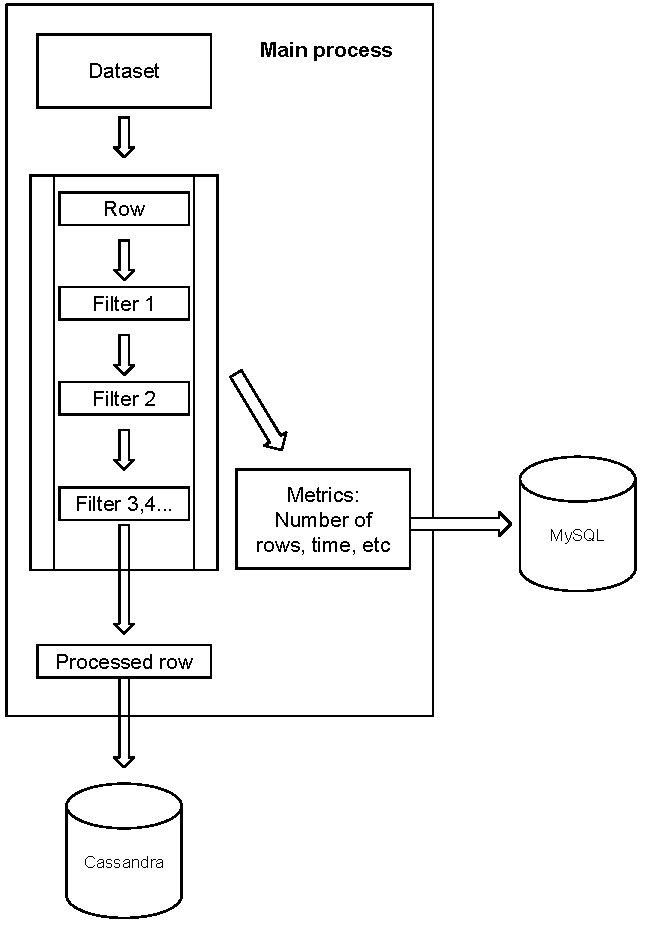
\includegraphics[width=120mm]{figures/program_overview_sequential.pdf}
  \caption[Sequential program overview.]{Sequential program overview.}
  \label{fig:sequential_program_overview}
\end{figure}

\section{Sequential program profiler analysis} \label{section:sequential_profiler}
The result of running \code{cProfile} on the sequential transformation program can be found in figure \ref{fig:sequential_profiler}. The dataset used had
27877 rows, 46 columns, and belonged to the extra overhead file format family.
Function calls with very low cumulative time have been omitted. In the profiling result, \code{ncalls} is the number of times the function was called,
\code{tottime} is total time spent in the function (excluding subfunctions), \code{cumtime} is the total time spent in the function
including its subfunctions, and \code{percall} is the quotient of \code{cumtime} divided by primitive calls \cite{26_2tppp2d}.

\begin{figure}[ht]
  \begin{VerbatimInput}{figures/profiling_17_may_short.txt}
    \caption[Sequential program \code{cProfile} output.]{Sequential program \code{cProfile} output. The most interesting functions (\code{process},
    \code{process\_record}, \code{post\_process\_record}, \code{consume\_record}, and \code{prepare}) are highlighted in green.}
  \label{fig:sequential_profiler}
\end{VerbatimInput}
\end{figure}

%\begin{figure}[ht]
%  \lstinputlisting[basicstyle=\tiny]{figures/profiling_17_may_short.txt}
%  \caption{Sequential program \code{cProfile} output}
%  \label{fig:sequential_profiler}
%\end{figure}

From the profiling information above, it is clear that some function calls take significantly more time than others, and are therefore
interesting targets for parallelization analysis. The \code{process} method is the one that launches the main pipeline that applies all
filters and performs the transformation of the dataset. The fact that it takes 66.280 seconds out of 66.567 is therefore expected. Among
the functions that \code{process} calls, \code{process\_record}, \code{post\_process\_record}, \code{consume\_record}, and \code{\_prepare} are the most
interesting. Other functions with relatively high cumulative time are called from these functions.
\begin{itemize}
  \item \code{process\_record} -- In the profiling information, \code{process\_record} appears twice, once in the file \code{pipeline.py} and once in the file
    \code{mappings.py}. The version in \code{pipeline.py} is abstract, with an implementation in each of the filters. It is evident that the implementation
    that is most common resides in \code{mappings.py} as it is the only one that shows up among the function calls that take up a significant amount of time.
    This is expected, as \textit{Mapping} is the most common filter and represented in \code{mappings.py}. The function has a low \code{percall} and a high
    \code{ncalls}, indicating that the reason it takes up a large portion of the total time is the fact that it is called many times due to the many filters
    and dataset rows. \code{process\_record} takes up 35.0\% of the total execution time.
  \item \code{post\_process\_record} -- Similarly to \code{process\_record}, \code{post\_process\_record} is an abstract method and is implemented in all filters.
    It also has a low \code{percall} and a high \code{ncalls}. \code{post\_process\_record} takes up 33.1\% of the total time.
  \item \code{consume\_record} -- This method calls \code{\_write\_record}, which is the method that writes rows to Cassandra after they have been transformed.
    \code{consume\_record} is called once per row and takes 8.4\% of the total time, and \code{\_write\_record} is responsible for 7.9\% of these. 
  \item \code{\_prepare} -- Called once before the program starts iterating over all rows, performing setup needed to perform the transformations properly.
    It has a relatively high \code{percall} and takes up 3.3\% of the total execution time.
\end{itemize}
The time spent in the functions above is 87.7\% of the toal time, and the majority of the rest of the code in \code{process} is contained in the body of the loop that iterates
over and performs actions on every row. Since only \code{\_prepare} runs before the loop, and a small portion of code is run after the loop, about 4\% of the code 
is run outside the loop. This means that around 96\% of the code is conceivably parallelizable, depending on the filters in the dataset's file format.\\

The following conclusions can be made from the analysis above:

\begin{itemize}
  \item A majority of the functions responsible for most of the time consumption have low \code{percall} and high \code{ncalls}, indicating that no single function is
    a significant bottleneck, and that the major reason these functions take up large portions of the total time is that they are called a high number of times.
  \item A relatively small portion of the code is spent in functions that perform I/O, indicating that the program is CPU bound and suitable for speedup using
    \code{multiprocessing}.
  \item Close to all of the code in \code{process} is run for each row, indicating that performing the transformation of different rows in different tasks is a
    suitable granularity when implementing the parallelization.
  \item The fact that \code{\_prepare} takes up a non-negligible part of the program and is called before the processing of each row, it may introduce extra overhead
    when parallelizing, since it may need to be called for each worker.
\end{itemize}

\section{Performance model calculations} \label{performance_model_calculations}
In this section, different performance calculation models are used to find a preliminary indication of possible speedup.

\subsection{Amdahl's law}
In the sequential profiling session, it is suggested that around 96\% of the code is parallelizable. The computer used for testing has 8 cores,
which is the value that will be used for the $n$ value when applying Amdahl's law to the profiling session run:

\begin{displaymath}
  S = \frac{1}{1 - 0.96 + \frac{0.96}{8}} = 6.25
  \label{fig:amdahl_calculation}
\end{displaymath}

\noindent This potential speedup of 6.25 does not take into account overhead associated with parallelization.

\subsection{Gustafson's law}
With Gustafson's law, the speedup is calculated as the following:

\begin{displaymath}
  S = 8 + (1-8) * 0.04 = 7.72
\end{displaymath}

\noindent With the more optimistic Gustafson's law, the speedup is higher. Overhead is not taken into account in the above calculation.

\subsection{Work-span model}
As mentioned in section \ref{work-span}, the increase in work when parallelizing a program should be kept to a minimum.
In addition, the span should be kept as small as possible. In the implementation made in this thesis, both the work and the span is increased.
The work is increased since the code that is run before the loop over each row has to be run once for each worker, and because the caching of
column mappings is done for each worker. The span is increased because of the added post processing needed when transforming datasets from the
extra overhead file format family. This suggests that parallelization cannot be utilized at its fullest, which may impact the speedup.

\section{Analysis of filter parallelizability}
Since the filters specify what the processing program should do to each row in a dataset, ``row by row'' or possibly chunks of rows is a suitable
granularity when implementing the parallelization of the program. Consequently, the filters of a file format are the prime candidates
for parallelization analysis. The analysis made is similar to the methodology used to identify the span in the work-span model described in
section \ref{work-span}. When applying the model to the problem of analyzing filters, a task is the processing of one row. In order to find
the tasks that need to be completed before other tasks, the filters that result in state that is accessed by subsequent rows or otherwise
affect the total processing of the dataset need to be identified.

Examining the filters, it is apparent that \textit{Dataset translation}, \textit{Null translation}, \textit{Relation currency},
\textit{Third party automapper}, \textit{Set value}, \textit{RegExp extract}, and \textit{RegExp replace} only operate on the current dataset row, with no side effects.
This means that they produce no state changes that affect subsequent rows, which means that they do not affect the parallelizability of a dataset.

Additionally, \textit{Dataset information}, \textit{Tradefile information}, \textit{Temporary variable}, \textit{Logger}, and \textit{Skip row} perform
operations that either pull information from resources that are available to all rows, or produce an effect that does not affect any other rows.
The \textit{Conditional block} filter only produces effects according to its subfilters (a set of the filters already mentioned), and does not affect parallelization by itself.
\\\\
Hence, the filters that can affect the parallelization of a dataset are:
\begin{itemize}
  \item \textit{Mapping}, since the trade id mapping may need to keep track of state that can be accessed in subsequent rows in order to make all id:s unique.
  \item \textit{Header detection}, since all rows beneath the (first) header row depend on the column names for mappings and other values.
  \item \textit{Global variable}, since the variable may be written and accessed by any subsequent rows. Each rewrite of the variable needs to happen before the next rewrite,
    in the original, sequential order if the verification result is to be correct.
  \item \textit{State variable}, for the same reasons as Global variable.
  \item \textit{Stop processing}, if one thread sees a conditional fulfilled and stops processing, it is possible for another thread to keep processing rows that are intended
    to be ignored, thereby violating the constraints.
\end{itemize}

\section{Code inspection}
After an initial code and file format inspection, the following conclusions where made:
\begin{itemize}
  \item The \textit{Header detection} filter is effectively performed only once, as it is ignored for all rows after the one where the header was found.
  \item The filters \textit{Global variable} and \textit{State variable} make the processing of every row depend on the previous, as the writing of the variables may happen on each row.
  \item The process of making an ID unique could possibly be broken out to a post processing step.
  \item All file formats contain \textit{Header detection}, and many contain the make unique feature of the trade ID mapping.
  \item There are many file formats that do not have either \textit{Global variable}, \textit{State variable} or \textit{Stop processing} among their filters.
\end{itemize}

The conclusions above indicate that header detection may be done before creating the parallel processes, sending this data to each process when they are created.
If the process of producing unique ID:s is then done as a post processing step, the following task DAGs illustrate how the dependencies when processing different
file formats appear: In figure \ref{fig:embarrassing_dag}, the task DAG for a file format without a Global variable or State variable filter is illustrated.
In figure \ref{fig:embarrassing_dag}, the task DAG for a file format containing a Global variable is illustrated. Since the span is equal to the work
in the file formats containing Global variables or State variables, parallelization of datasets with these formats will result in no speedup according to the %Illustrate work-span?
work-span model (as $T_1 \leq T_\infty \Rightarrow S \leq 1$). File formats containing \textit{Stop processing} make it unfeasible to produce correct verification results
when parallelizing. Determination of whether the result is correct is non-viable if any rows are processed in different processes (as rows that should not be included in the result may be included anyway).

\begin{sidewaysfigure}[ht]
  \centering
  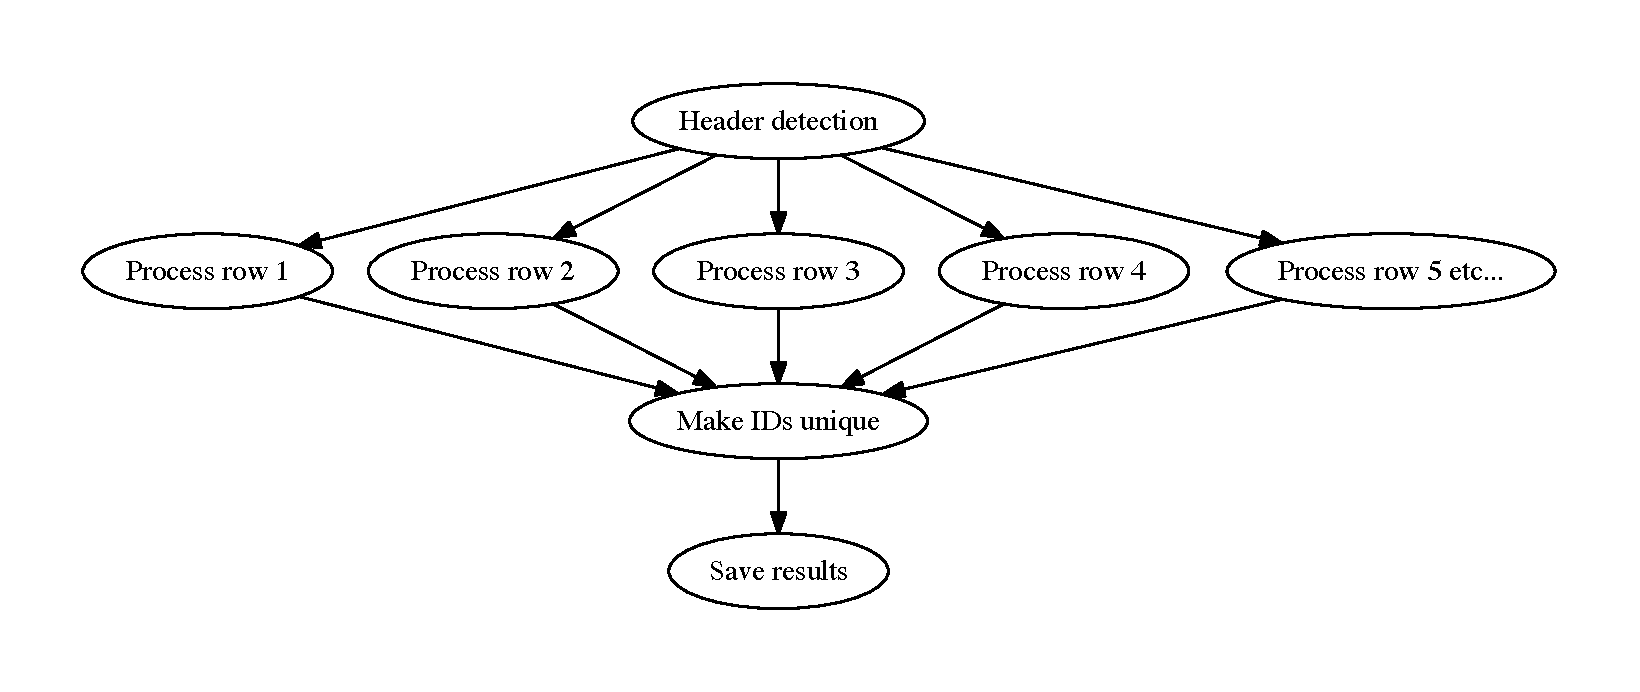
\includegraphics[width=200mm]{figures/embarrassing_file_format.pdf}
  \caption[Task DAG for a file format that does not contain global or state variables.]{An example of a task DAG for a file format that does not contain global variable or state variables. Header detections needs
  to be performed up front, and making trade IDs unique needs to be performed in a post processing step. The processing of each row does not depend on each other.}
  \label{fig:embarrassing_dag}
\end{sidewaysfigure}

\begin{figure}[ht]
  \centering
  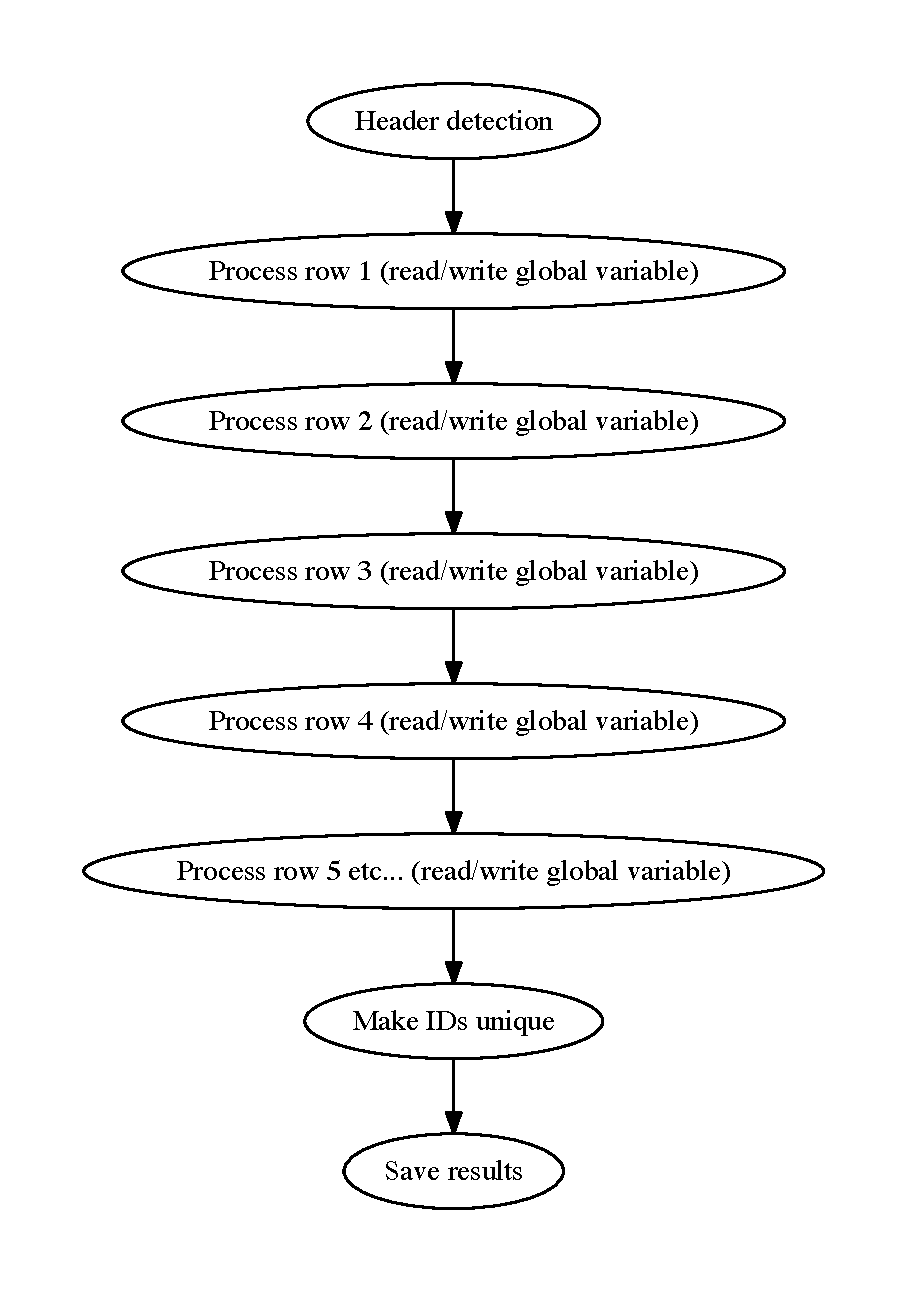
\includegraphics[width=120mm]{figures/global_variable_file_format.pdf}
  \caption[Task DAG for a file format that contains global or state variables.]{An example of a task DAG for a file format that contains global or state variables. Since each row may read and
  write the global (or state) variable, every task depends on the previous task.}
  \label{fig:global_dag}
\end{figure}

\section{Filter families}
With the help of the findings from the previous sections, families of filters with different characteristics can be identified.

\begin{itemize}
\item \textbf{Embarrassingly parallel filters} --
The filters that do not affect parallelization in any way are:
\textit{Dataset translation}, \textit{Null translation}, \textit{Relation currency},
\textit{Third party automapper}, \textit{Set value}, \textit{RegExp extract}, \textit{RegExp replace},
\textit{Dataset information}, \textit{Tradefile information}, \textit{Temporary variable}, \textit{Logger}, \textit{Skip row}, and \textit{Conditional block}.
In addition, \textit{Mapping} is included among these filters if the make unique feature is disabled.
\item \textbf{Overhead filters} -- 
Filters that introduce parallelization overhead are: \textit{Mapping} (if the make unique feature is enabled) and \textit{Header detection}.
\item \textbf{Inherently serial filters} --
The filters that enforce serial execution of the entire transformation are: \textit{Global variable}, \textit{State variable}, and \textit{Stop processing}.
\end{itemize}

\section{File format families}
In addition to the filter families, the fact that the \textit{Header detection} filter is present in all file formats makes it possible to identify the following
file format families relevant to this thesis:

\begin{itemize}
\item \textbf{Embarrassingly parallel file formats} --
  File formats that with the exception of \textit{Header detection} contain only embarrassingly parallel filters. 
\item \textbf{Extra overhead file formats} --
  Formats that in addition to \textit{Header detection} and a number of embarrassingly parallel filters also contain \textit{Mapping} with the make unique filter enabled.
\item \textbf{Inherently serial file formats} --
  Formats that contain any of the inherently serial filters.
\end{itemize}

\section{Parallelization}
In accordance with section \ref{related_work}, the Python \code{multiprocessing} module was used to implement the parallelization of the program. Additionally, measures where taken to send as little
data as possible between processes and to avoid introducing excessive complexity to the codebase. The \code{multiprocessing.Queue} facility was chosen for communication between processes due to its
noted performance and built-in synchronization \cite{singh_2013_parallel_padpwprfmm}.

Before deciding to use the parallelized version of program, the list of filters in a file format is examined for any of the inherently serial filters
\textit{Global variable}, \textit{State variable}, or \textit{Stop processing}. If any of these are found, the
program falls back to its sequential version. Otherwise, the program carries on in accordance with figure \ref{fig:embarrassing_dag}. First, before creating any additional processes, the Header detection filter
is applied row by row until it produces a result (commonly after a few rows). Next, a (tunable) number of processes, as well as two queues are created. A number of row spans, or chunks, are then created by splitting
the rows beneath the header row into equally sized partitions. The first queue is used to transfer the data needed to process a chunk of the dataset, including the header data, the row span, and the result metadata.
In order to avoid errors and sending large objects between processes, only the primary key used to retrieve the result metadata object from the MySQL database is sent to the processes.
After this, the processes can independently retrieve the data. The second queue is used for sending the partial metrics objects for each chunk, and for indicating if a process is done processing
its data or if it encountered an error. Since all other results are written to the Cassandra database, this is the only information that needs to be sent to the main process. The queues can be
denoted the 'chunk queue' and the 'message queue', respectively.

In each of the created processes, the rows in the chunk are retrieved from the Cassandra database and a new object containing metrics for the chunk is created. The chunk is then processed as in the sequential program,
applying all filters to each row. The metrics object is updated during the processing, as in the original program. If the chunk was processed correctly, the metrics object is put on the message queue. Otherwise,
if an exception occurs, an error message is put on the queue instead. When all data in a process has finished processing, a message indicating that the process has finished its work is put on the message queue.

The main process continuously polls the message queue, and merges the partial metrics objects as they are polled from the queue. If an error message is encountered, an exception is raised on the main thread, mimicking the
behavior of the original sequential program. It also increments a counter whenever a done message is received from a process. When the counter is equal to the number of subprocesses, the main process stops waiting
for messages, and progresses with the post processing step of making the trade ID:s unique. Finally, the main process saves the result object with the corresponding merged metrics to the MySQL database. At this point,
the program has produced a finished verification result.

A simplified overview of the parallel program can be found in figure \ref{fig:parallel_program_overview}.

\begin{sidewaysfigure}[ht]
  \centering
  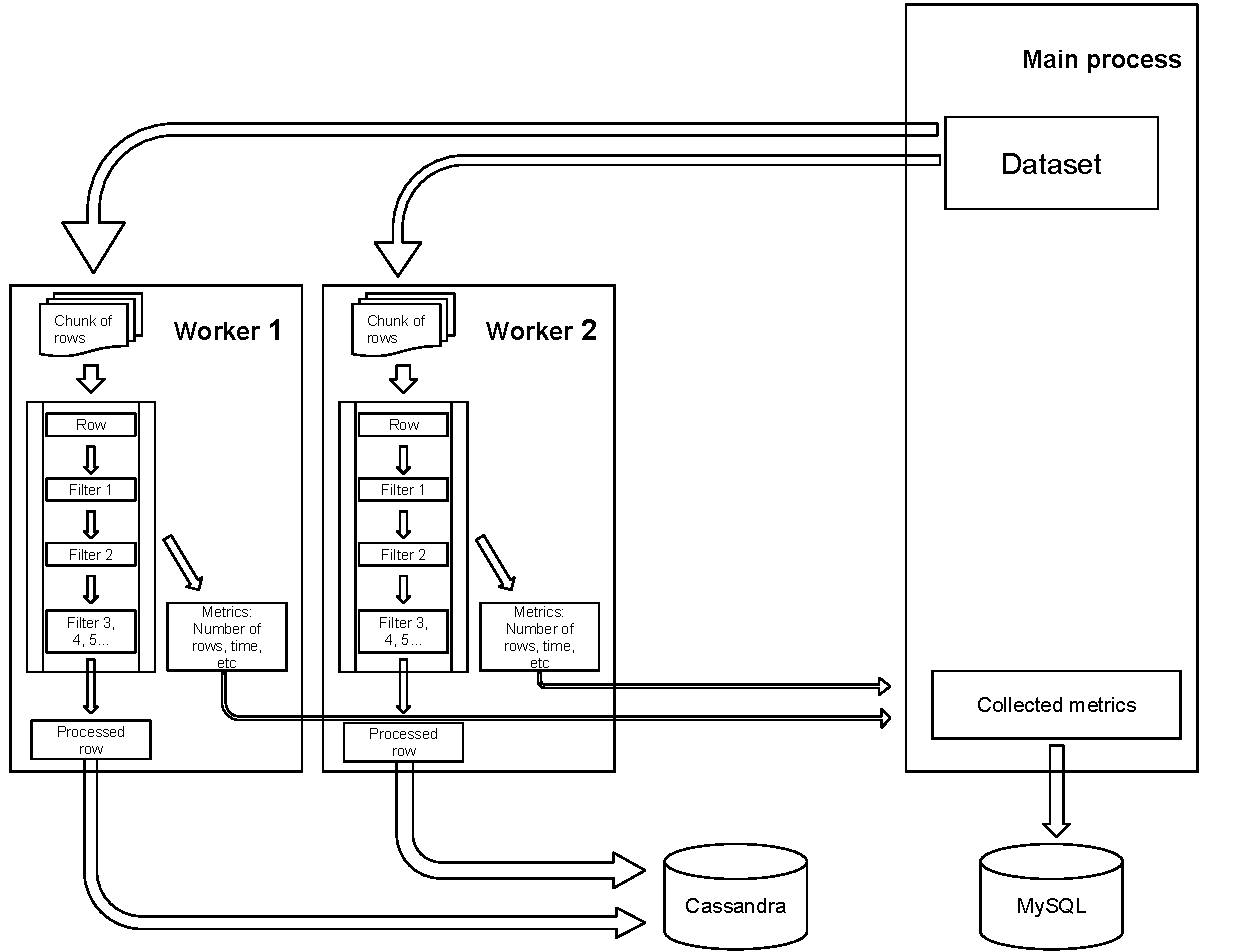
\includegraphics[width=200mm]{figures/program_overview.pdf}
  \caption[Parallel program overview.]{Parallel program overview.}
  \label{fig:parallel_program_overview}
\end{sidewaysfigure}

\section{Sources of overhead}
During the implementation of the parallel version of the program, the following possible sources of parallelization overhead where identified:

\begin{itemize}
  \item The \code{multiprocessing} module, where creating processes and transferring data between processes is costly.
  \item Less effective caching of mappings. Since the mappings cache is local to each subprocess, caches are built up individually. This results in fewer cache hits than in the sequential program, and more total work
    looking up values in the MySQL database. Hardware cache may also be affected in a similar manner.
  \item The process of making trade ID:s unique is added as an extra step after the main data processing pipeline.
  \item Because they lack built-in support for multiprocessing, the Python connections between both MySQL and Cassandra need to be restarted in the startup of each subprocess.
  \item \code{\_prepare} has to be called once for each of the workers, compared to only one call for the sequential program.
\end{itemize}


\chapter{Benchmark Environment}
    In this section, the experiments and the hardware used to conduct them are desribed.

\section{Hardware}
%\subsection{Initial testing laptop}
%For initial working, testing, and profiling, a laptop computer with several cores was used. The laptop is a MacBook Pro running OSX, with an Intel Core i7 processor and 4 physical cores.
%The processor supports hyperthreading, bringing the number of logical cores to 8.
For the main evaluation, TriOptima’s acceptance test environment with hardware similar to what is used in production, was used. This is a stationary computer running Linux CentOS,
with a dual processor architecture. The processors are 2 Intel Xeon E5504 processors with 4 cores each, making a total of 8 cores. The cores do not support hyperthreading.

\section{Test datasets}
For all datasets, the number of filters is limited to a few more than the number of columns, as the majority of the filters are column mapping filters.
This is typical for most datasets, making this a suitable sample of datasets. No datasets with inherently serial file formats where used, as these cannot be
parllelized and would provide no interesting data. Instead, the focus of the experiments are on the \textit{Extra overhead} file formats, since these are the
most common (since making trade ID:s unique is a useful feature). They also give the fairest indication of how successful the parallelization is, as they are
both the worst case (apart from inherently serial file formats) and the common case. Another reason why this set of datasets was chosen is their differing sizes,
with potentially differing parallelization benefits.

The characteristics of the test datasets are outlined in figure \ref{fig:test_datasets}.

%\subsection{Large}
%\begin{itemize}
  %\item \textbf{Rows:} 338,730
  %\item \textbf{Columns:} 89
  %\item \textbf{File format family:} Extra overhead
%\end{itemize}
\begin{figure}[ht]
\centering
\begin{tabular}{|l|l|l|l|}
\hline
Dataset & Rows   & Columns & File format family \\ \hline
Tiny    & 102    & 46      & Extra overhead     \\ \hline
Small   & 2,890  & 46      & Extra overhead     \\ \hline
Medium  & 23,763 & 46      & Extra overhead     \\ \hline
Large  & 349309 & 41      & Extra overhead     \\ \hline
\end{tabular}
\label{fig:test_datasets}
\caption{Test datasets.}
\end{figure}

\section{Experiments}
\subsection{Benchmarks}
For each dataset, experiments where run to gather information about time and memory consumption for different configurations.
The experiments entailed performing a dataset transformation using the parallel program with each number of workers in the range 1 to 2 times the number of cores: 1--16.
In addition to running the parallel program, a serial transformation was also performed as a reference point.
In each of the experiments, the Python \code{resource} module was used in each worker process to find the user time, system time, and maximum memory consumption.
These values where then summed in order to find the total resource use. In the case of maximum memory consumption, this means that the number found is a worst case
number. It is possible that the processes in total have a smaller maximum memory consumption since they may reach their maximum memory consumption at different
points in time.

In order to provide more accurate results, the experiments where run 10 times for each dataset--worker number configuration. These 10 runs where then used to calculate the
average value as well as the standard deviation for each metric value. In addition, the speedup was calculated by dividing the sequential execution time with the parallel execution
time for each worker value.

\subsection{Profiling}
For each dataset, a single run with 8 workers was profiled using \code{cProfile} in order to find where in the program the most time is spent. This was done in order
to better understand the benchmark results.

\chapter{Results}
    \section{Parallel program profiler analysis}
After the parallel program implementation, another round of profiling using \code{cProfile} was conducted. This was done on the initial testing laptop,
with 4 workers, on the same dataset as the first round of profiling. The results from the main process that orchestrates the other processes and aggregates their results can be
found in \ref{fig:parallel_profiler_main}. The results from two of the workers can be found in figure \ref{fig:parallel_profiler_w1} and figure \ref{fig:parallel_profiler_w2}.

For the main process, it is apparent that \code{post\_process\_parallel}, the function that makes the trade ID:s unique after the parallel worker processes have finished
executing, adds non-negligible overhead. \code{aggregate\_result} contains the code that creates the other processes and waits for these to produce their partial results,
aggregating them as they are produced. This code takes up 84\% of the total time, while the remaining 16\% of the code is effectively overhead.
In addtion, as mentioned in section \ref{section:sequential_profiler} as a possibility, \code{\_prepare} is called for each
worker process, resulting in extra overhead. It is conceivable that these sources of overhead are less noticable when processing a larger dataset, as the effects of
the functions that are called only one time take up a smaller amount of the total running time if the dataset contains a larger number of rows.

For the worker processes, the results are similar to the results from profiling the sequential program in section \ref{section:sequential_profiler}, but with lower
\code{cumtime} values. This is expected due to the lower number of rows per worker. The same functions as in the sequential program are responsible for the largest
portion of the running time, \code{process\_record}, \code{post\_process\_record}, \code{consume\_record}, and \code{\_prepare}.

\begin{figure}[ht]
  \lstinputlisting[basicstyle=\tiny]{figures/profiling_parallel_19_may_main.txt}
  \caption{Main process in parallel program \code{cProfile} output}
  \label{fig:parallel_profiler_main}
\end{figure}
\clearpage

\begin{figure}[ht]
  \lstinputlisting[basicstyle=\tiny]{figures/profiling_parallel_19_may_31147.txt}
  \caption{Worker 1 in parallel program \code{cProfile} output}
  \label{fig:parallel_profiler_w1}
\end{figure}
\clearpage

\begin{figure}[ht]
  \lstinputlisting[basicstyle=\tiny]{figures/profiling_parallel_19_may_31148.txt}
  \caption{Worker 2 in parallel program \code{cProfile} output}
  \label{fig:parallel_profiler_w2}
\end{figure}
\clearpage

\section{Transformation benchmarks}
The benchmarks for the experiments are outlined below. For each dataset, the results consist of a table containing
speedup, real time, user time, system time, and memory usage for each worker number. The standard deviation is represented
as a value following the $\pm$ sign. The value S in worker column signifies the original sequential program, while 1 is the
parallel program with a single worker. In addition to the tables, the real time, speedup, and memory usage are illustrated
using plots in order to visually demonstrate how the values change with the number of workers. In the plots for real time
and memory usage, the standard deviation is illustrated using black bars above and below each data point\footnote{
The standard deviation is shown for all plots of real time and memory usage, but it may be too small to be seen for some of the plots.}.

\section{Dataset 1}
The results for dataset 1 can be found in figures \ref{fig:dataset_1_table}, \ref{fig:dataset_1_real_time}, \ref{fig:dataset_1_speedup}, and \ref{fig:dataset_1_memory}.

\begin{figure}[ht]
\centering
\resizebox{\linewidth}{!}{%
\begin{tabular}{|c|c|c|c|c|c|}%
  \hline
  \bfseries Workers & \bfseries Speedup & \bfseries Real (s) & \bfseries User (s) & \bfseries System (s) & \bfseries Memory usage (MB)
  \csvreader[respect all,head to column names]{figures/dataset_1/dataset_1_table.csv}{workers=\w,speedup=\spd,real=\r,user=\u,system=\s,memory_usage_mb=\m}
  {\\\hline \w & \spd & \r & \u & \s & \m}
  \\ \hline
\end{tabular}}
\caption[Dataset 1 benchmark table.]{Dataset 1 benchmark table. The table displays the number of workers, the speedup (sequential run real time divided by real time), real time,
user time, system time, and memory usage. The standard deviation is displayed with a value following the $\pm$ sign.}
\label{fig:dataset_1_table}
\end{figure}

\begin{figure}[ht]
  \centering
  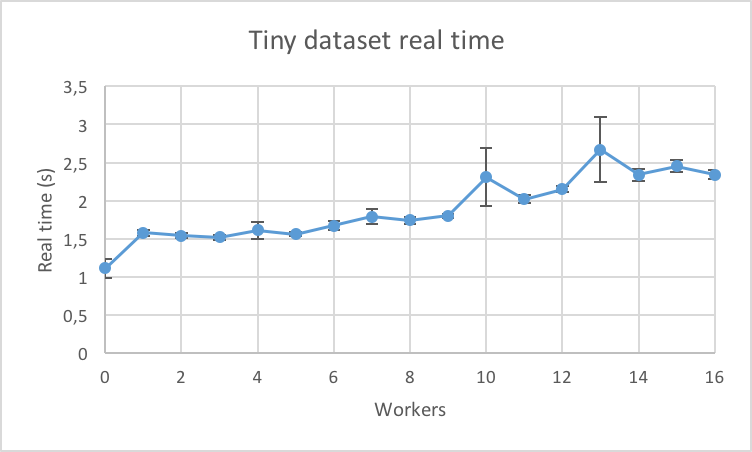
\includegraphics[width=120mm]{figures/dataset_1/dataset_1_real_time.png}
  \caption[Real time plot for dataset 1.]{Real time plot for dataset 1. The X axis shows the number of workers, where 0 signifies the sequential program run.
  The Y axis shows the real execution time for each worker value. The standard deviation is displayed with black bars around each data point. Real time
  increases as number of workers increase. The data points at 10 and 13 workers show high standard deviation.}
  \label{fig:dataset_1_real_time}
\end{figure}

\begin{figure}[ht]
  \centering
  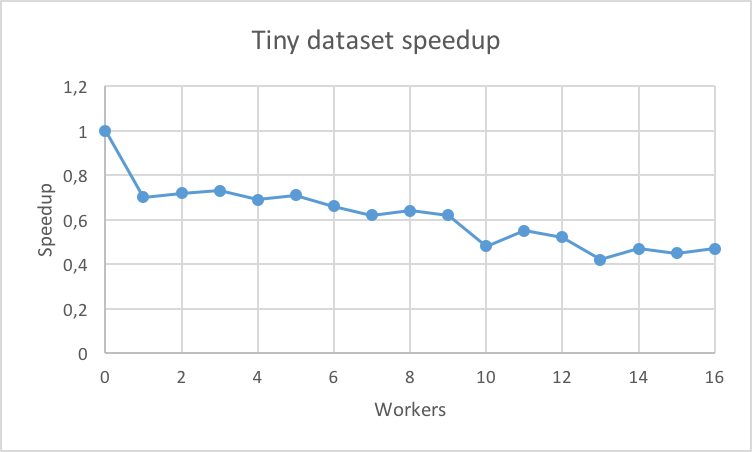
\includegraphics[width=120mm]{figures/dataset_1/dataset_1_speedup.png}
  \caption[Speedup plot for dataset 1.]{Speedup plot for dataset 1. The X axis shows the number of workers, and the Y axis shows a scalar value signifying the speedup as
  ``number of times faster than sequential execution''. Speedup decreases with each added worker, down to about half the speed of the sequential execution.}
  \label{fig:dataset_1_speedup}
\end{figure}

\begin{figure}[ht]
  \centering
  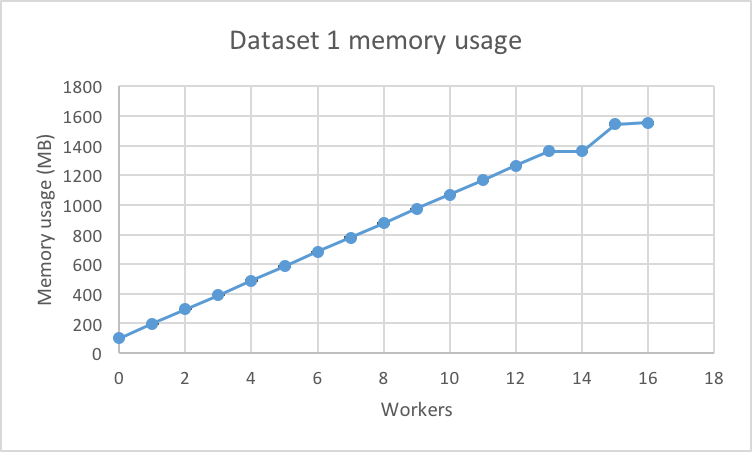
\includegraphics[width=120mm]{figures/dataset_1/dataset_1_memory.png}
  \caption[Memory usage plot for dataset 1.]{Memory usage plot for dataset 1. The X axis shows the numner of workers, and the Y axis shows the total memory usage as
  a sum of the highest memory usage for each worker process, in addition to the main process. Memory usage increases close to linearly with each added worker,
  up to about 1.6 GB for 16 workers.}
  \label{fig:dataset_1_memory}
\end{figure}

\section{Dataset 2}
The results for dataset 2 can be found in figures \ref{fig:dataset_2_table}, \ref{fig:dataset_2_real_time}, \ref{fig:dataset_2_speedup}, and \ref{fig:dataset_2_memory}.

\begin{figure}[ht]
\centering
\resizebox{\linewidth}{!}{%
\begin{tabular}{|c|c|c|c|c|c|}%
  \hline
  \bfseries Workers & \bfseries Speedup & \bfseries Real (s) & \bfseries User (s) & \bfseries System (s) & \bfseries Memory usage (MB)
  \csvreader[respect all,head to column names]{figures/dataset_2/dataset_2_table.csv}{workers=\w,speedup=\spd,real=\r,user=\u,system=\s,memory_usage_mb=\m}
  {\\\hline \w & \spd & \r & \u & \s & \m}
  \\ \hline
\end{tabular}}
\caption[Dataset 2 benchmark table.]{Dataset 2 benchmark table. The table displays the number of workers, the speedup (sequential run real time divided by real time), real time,
user time, system time, and memory usage. The standard deviation is displayed with a value following the $\pm$ sign.}
\label{fig:dataset_2_table}
\end{figure}

\begin{figure}[ht]
  \centering
  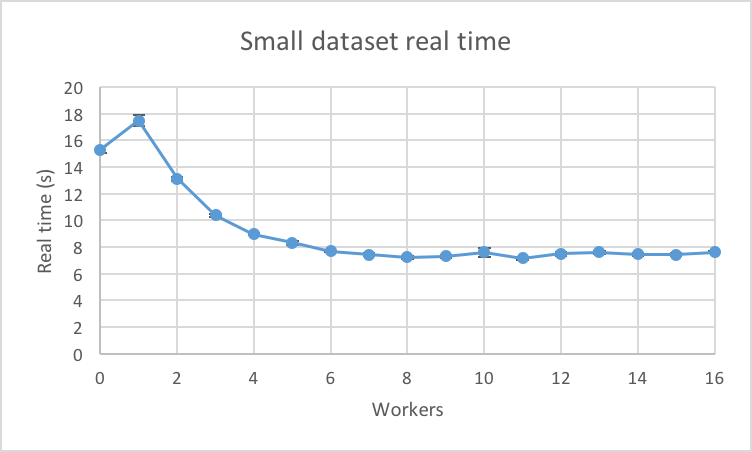
\includegraphics[width=120mm]{figures/dataset_2/dataset_2_real_time.png}
  \caption[Real time plot for dataset 2.]{Real time plot for dataset 2. The X axis shows the number of workers, where 0 signifies the sequential program run.
  The Y axis shows the real execution time for each worker value. The standard deviation is displayed with black bars around each data point. The real time
  decreases with each added worker up to 8 workers, where it evens out. The decrease in real time for each added worker becomes smaller as the number increases.}
  \label{fig:dataset_2_real_time}
\end{figure}

\begin{figure}[ht]
  \centering
  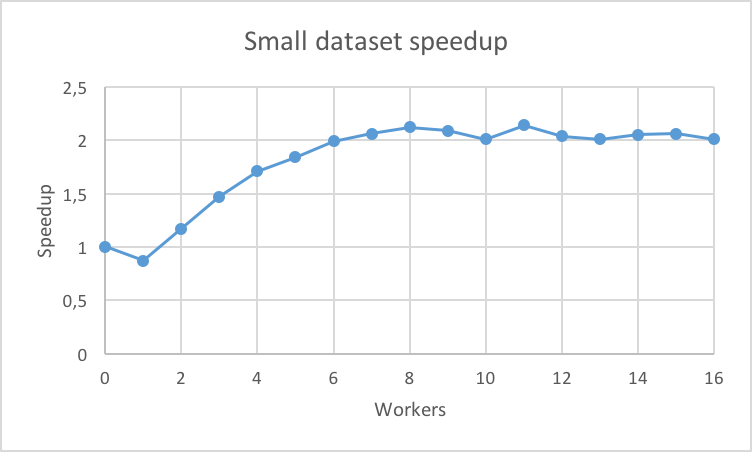
\includegraphics[width=120mm]{figures/dataset_2/dataset_2_speedup.png}
  \caption[Speedup plot for dataset 2.]{Speedup plot for dataset 2. The X axis shows the number of workers, and the Y axis shows a scalar value signifying the speedup as
  ``number of times faster than sequential execution''. Speedup increases with each worker, evening out around 8 workers and 2.1X speedup.}
  \label{fig:dataset_2_speedup}
\end{figure}

\begin{figure}[ht]
  \centering
  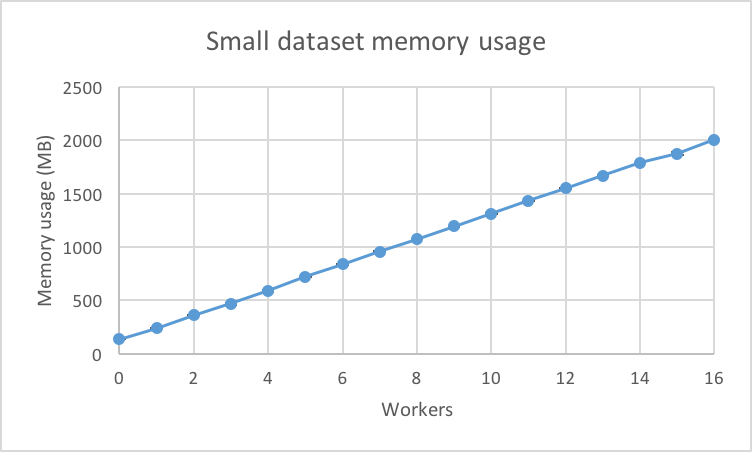
\includegraphics[width=120mm]{figures/dataset_2/dataset_2_memory.png}
  \caption[Memory usage plot for dataset 2.]{Memory usage plot for dataset 2. The X axis shows the numner of workers, and the Y axis shows the total memory usage as
  a sum of the highest memory usage for each worker process, in addition to the main process. Memory usage increases close to linearly with each added worker,
  up to about 2 GB for 16 workers.}
  \label{fig:dataset_2_memory}
\end{figure}

\section{Dataset 3}
The results for dataset 3 can be found in figures \ref{fig:dataset_3_table}, \ref{fig:dataset_3_real_time}, \ref{fig:dataset_3_speedup}, and \ref{fig:dataset_3_memory}.

\begin{figure}[ht]
\centering
\resizebox{\linewidth}{!}{%
\begin{tabular}{|c|c|c|c|c|c|}%
  \hline
  \bfseries Workers & \bfseries Speedup & \bfseries Real (s) & \bfseries User (s) & \bfseries System (s) & \bfseries Memory usage (MB)
  \csvreader[respect all,head to column names]{figures/dataset_3/dataset_3_table.csv}{workers=\w,speedup=\spd,real=\r,user=\u,system=\s,memory_usage_mb=\m}
  {\\\hline \w & \spd & \r & \u & \s & \m}
  \\ \hline
\end{tabular}}
\caption[Dataset 3 benchmark table.]{Dataset 3 benchmark table. The table displays the number of workers, the speedup (sequential run real time divided by real time), real time,
user time, system time, and memory usage. The standard deviation is displayed with a value following the $\pm$ sign.}
\label{fig:dataset_3_table}
\end{figure}

\begin{figure}[ht]
  \centering
  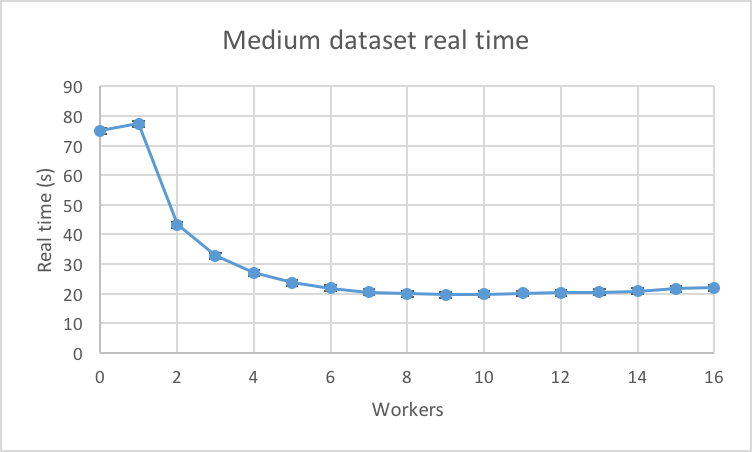
\includegraphics[width=120mm]{figures/dataset_3/dataset_3_real_time.png}
  \caption[Real time plot for dataset 3.]{Real time plot for dataset 3. The X axis shows the number of workers, where 0 signifies the sequential program run.
  The Y axis shows the real execution time for each worker value. The standard deviation is displayed with black bars around each data point. The real time
  decreases with each added worker up to 8 workers, where it evens out. The decrease in real time for each added worker becomes smaller as the number increases.}
  \label{fig:dataset_3_real_time}
\end{figure}

\begin{figure}[ht]
  \centering
  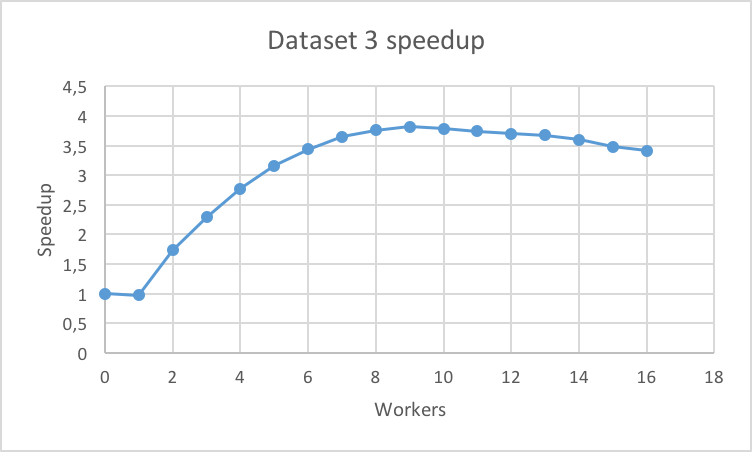
\includegraphics[width=120mm]{figures/dataset_3/dataset_3_speedup.png}
  \caption[Speedup plot for dataset 3.]{Speedup plot for dataset 3. The X axis shows the number of workers, and the Y axis shows a scalar value signifying the speedup as
  ``number of times faster than sequential execution''. Speedup increases with each worker, evening out around 8-9 workers and 3.8X speedup.}
  \label{fig:dataset_3_speedup}
\end{figure}

\begin{figure}[ht]
  \centering
  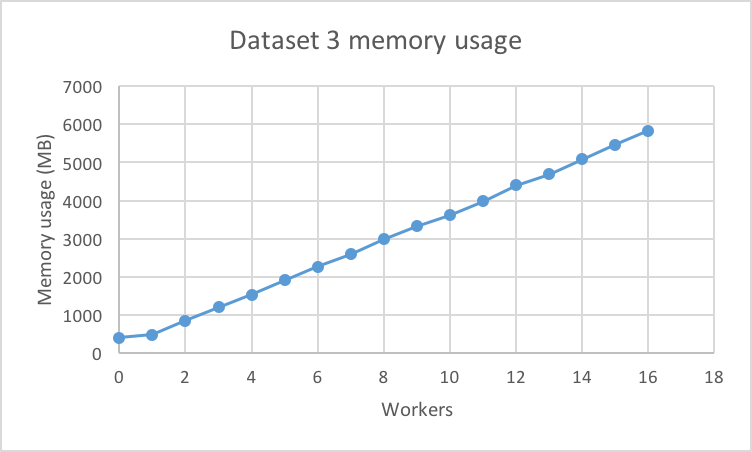
\includegraphics[width=120mm]{figures/dataset_3/dataset_3_memory.png}
  \caption[Memory usage plot for dataset 3.]{Memory usage plot for dataset 3. The X axis shows the numner of workers, and the Y axis shows the total memory usage as
  a sum of the highest memory usage for each worker process, in addition to the main process. Memory usage increases close to linearly with each added worker,
  up to about 6 GB for 16 workers.}
  \label{fig:dataset_3_memory}
\end{figure}


\section{Dataset 4}
The results for dataset 4 can be found in figures \ref{fig:dataset_4_table}, \ref{fig:dataset_4_real_time}, \ref{fig:dataset_4_speedup}, and \ref{fig:dataset_4_memory}.

\begin{figure}[ht]
\centering
\resizebox{\linewidth}{!}{%
\begin{tabular}{|c|c|c|c|c|c|}%
  \hline
  \bfseries Workers & \bfseries Speedup & \bfseries Real (s) & \bfseries User (s) & \bfseries System (s) & \bfseries Memory usage (MB)
  \csvreader[respect all,head to column names]{figures/dataset_4/dataset_4_table.csv}{workers=\w,speedup=\spd,real=\r,user=\u,system=\s,memory_usage_mb=\m}
  {\\\hline \w & \spd & \r & \u & \s & \m}
  \\ \hline
\end{tabular}}
\caption[Dataset 4 benchmark table.]{Dataset 4 benchmark table. The table displays the number of workers, the speedup (sequential run real time divided by real time), real time,
user time, system time, and memory usage. The standard deviation is displayed with a value following the $\pm$ sign.}
\label{fig:dataset_4_table}
\end{figure}

\begin{figure}[ht]
  \centering
  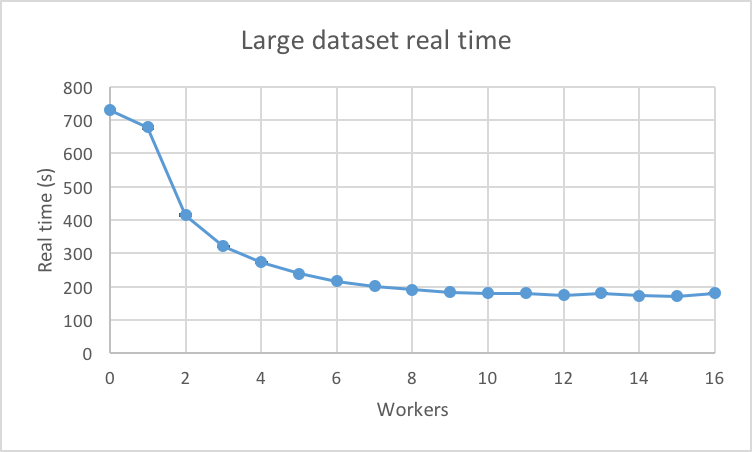
\includegraphics[width=120mm]{figures/dataset_4/dataset_4_real_time.png}
  \caption[Real time plot for dataset 4.]{Real time plot for dataset 4. The X axis shows the number of workers, where 0 signifies the sequential program run.
  The Y axis shows the real execution time for each worker value. The standard deviation is displayed with black bars around each data point. The real time
  decreases with each added worker up to 12 workers, where it evens out. The decrease in real time for each added worker becomes smaller as the number increases.}
  \label{fig:dataset_4_real_time}
\end{figure}

\begin{figure}[ht]
  \centering
  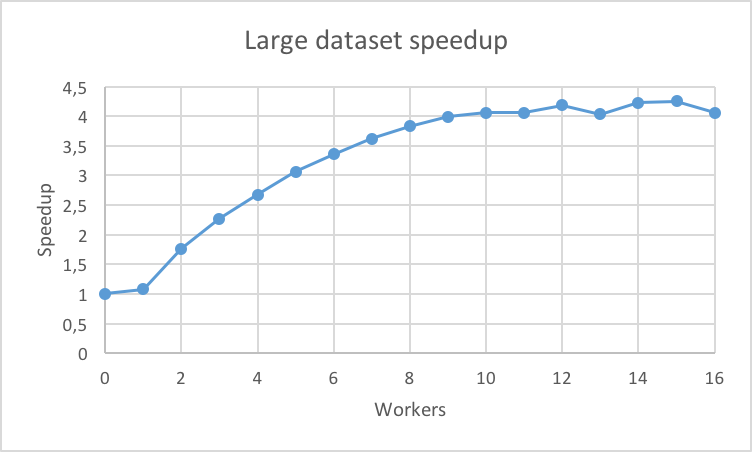
\includegraphics[width=120mm]{figures/dataset_4/dataset_4_speedup.png}
  \caption[Speedup plot for dataset 4.]{Speedup plot for dataset 4. The X axis shows the number of workers, and the Y axis shows a scalar value signifying the speedup as
  ``number of times faster than sequential execution''. Speedup increases with each worker, evening out around 12 workers and 4.2X speedup.}
  \label{fig:dataset_4_speedup}
\end{figure}

\begin{figure}[ht]
  \centering
  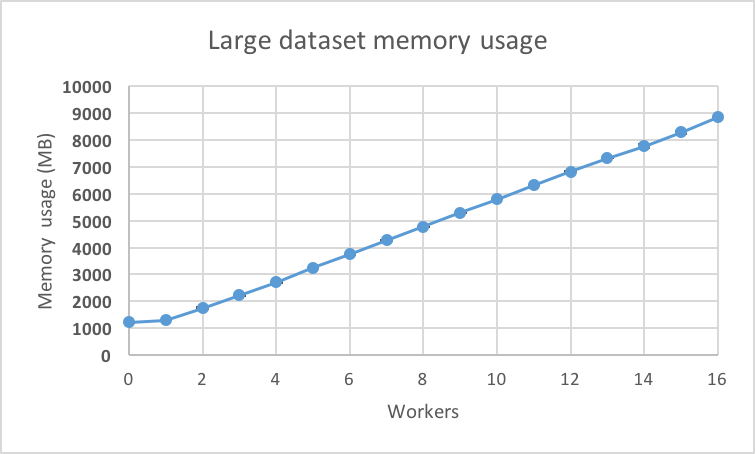
\includegraphics[width=120mm]{figures/dataset_4/dataset_4_memory.png}
  \caption[Memory usage plot for dataset 4.]{Memory usage plot for dataset 4. The X axis shows the numner of workers, and the Y axis shows the total memory usage as
  a sum of the highest memory usage for each worker process, in addition to the main process. Memory usage increases close to linearly with each added worker,
  up to about 8.8 GB for 16 workers.}
  \label{fig:dataset_4_memory}
\end{figure}


\chapter{Discussion \& Conclusions}
    The results in the previous chapter are discussed below, in an effort to explain them. In addition, final conclusions
about the thesis as a whole are drawn.

\section{Dataset benchmarks discussion}
\subsection{Tiny dataset discussion}
The tiny dataset shows poor results when parallelizing. For every worker number, only slowdown can be observed.
The real time values for 10 and 12 workers show high standard deviations when comparing with the average value. It is conceivable that
tasks such as creating processes have a more noticable impact for the low execution time.

The profiling session for the main process for the tiny dataset showed that \code{aggregate\_result} takes up 70\% of the time. Since this is the function
that performs the main parallel processing of the dataset, about 30\% of the execution time is overhead due to for example header detection
and making trade ID:s unique. Since \code{aggregate\_result} takes 0.4 seconds (15.7\% of execution time ) more to execute than it takes for a single worker to finish,
it appears as though parallelization and aggregating the partial results result in noticable overhead for the tiny dataset.
It is conceivable that the above results in the fact that only slowdown can be observed when parallelizing the tiny dataset.

Even without the parallel aggregation step, the tiny dataset still results in slowdown. A steady, close to linear increase in memory usage can be observed,
resulting in total memory usage several times above what is used for the sequential program.

\subsection{Small dataset discussion}
For the small dataset, some speedup scaling can be observed, with the maximum value around 2.1. As more workers are added, speedup is increased,
flattening out around 8 workers. This fits with the fact that the testing machine has 8 cores, effectively making it able to utilize 
true parallelism for a maximum of 8 workers. The impact of adding more workers decreases with each one that is added. In the profiling session
\code{post\_process\_parallel} is shown to take up a relatively large portion of the execution time (22.5\%). Since this function is a separate,
sequential and constant step, it is not affected by parallelization and therefore takes up varying percentages of the total time. Since more parallelization
leads to faster execution of the parallel portion of the code, the post processing becomes more significant as workers are added, contributing to the fact
that adding more workers results in less and less increase in speedup.

Without the post processing step, the small dataset gets slightly better speedup for 8 workers, 2.7X instead of 2.11X. This is still not close to
the performance model calculations, which can be seen as disappointing. The memory usage grows in a similar manner to the tiny dataset, though the values are greater.
Real time shows relatively low standard deviations compared to the total time, indicating that real time is fairly accurate for each worker
value.

\subsection{Medium dataset discussion}
The medium shows greater speedup than the small dataset, with a similar shape to the speedup by worker curve. The maximum speedup is
around 3.8, evening out around 8 workers, once again showing the best results around the machine's core number. This further suggests that larger
individal workload, this time a result of the larger dataset size, results in better speedup. Real time again shows
low standard deviation. Memory usage for the worker numbers with the largest speedup values is around 3 GB for dataset 3, demonstrating
that a large price in memory usage is paid for parallelization, which may impact performance negatively for large dataset sizes and
worker numbers.

The profiling session for the main process shows that \code{aggregate\_result} (30.138 s) takes a similar amount of time to the execution of
the worker processes (30.050 s). This suggests that parallelization overhead is not a major part of the execution time for the medium dataset.
However, in the worker process the \code{process} function (handling the main dataset processing) takes up 28.802 s of the total 30.050 s that the
worker takes to execute. This suggests a small overhead in the form of worker startup (4\%).
The post processing step takes up about 7.0\% of the execution time for 8 workers. This is less than for the small dataset, but may still contribute
to the fact that adding workers results in less increase in speedup.

Without the parallel processing, the medium dataset shows slightly better speedup for 8 workers. However, this increase is only from 3.76X to 4.04X
speedup, meaning that it still has relatively low efficiency.

\subsection{Large dataset discussion}
The large dataset shows an even greater speedup, maintaining the trend of larger parallelization gains for larger datasets. Speedup for the large
dataset increases past 8 workers, flattening out around 11 workers. From the profiling session, it is evident that workers for the larger dataset
may receive different workloads (taking between 412 seconds and 503 seconds) even though the chunks are the same size. This means that for 8 workers
(the same as the number of cores), several cores are unused as the faster workers terminate and the program waits for the slow workers to terminate.
By having more workers than cores, work can be more evenly scheduled among cores, resulting in better utilization of the processing power of the cores.

The profiling session also shows that \code{\_prepare} takes up less than 2\% of the processing time for the workers, meaning that workers for the large
dataset spend more time in the main row processing loop, likely contributing to the fact that the larger dataset shows greater speedup.

The post processing step takes up about 6.5\% of the execution time for 8 workers, close to the medium dataset. Without the parallel processing,
the large dataset shows slighlty better speedup for 8 workers. However, this increase is only from 4.3X to 4.6X speedup, meaning that it still has
relatively low efficiency.


%\subsection{Dataset 4}
%With the even larger dataset 4, another increase in speedup can be observed. Once again, the trend of greater parallelization gains for larger
%dataset sizes holds. Interestingly, speedup increases slightly even past 8 workers, though it flattens out around 12 workers.
%Though the program is largely CPU bound, the reason for the increase when using a number of workers greater than the number of cores may be
%greater CPU utilization when waiting for I/O when extra workers are added, as the chance of finding a worker with CPU bound work to do increases. 
%Real time standard deviation follows the same, stable trend also for dataset 4. Memory usage when parallelizing this significantly larger dataset,
%ranging between 5 GB and 7 GB for the worker values with the greatest speedup.

\subsection{General benchmark trends}
In general, user time increases significantly with added workers, as is expected due to the greater total CPU utilization. Together with the
fact that memory usage increases linearly with worker number, this indicates that a noteworthy amount of system resources is required 
for parallelization as dataset sizes and number of workers grow large. The highest amount of memory used by the program is 7.7 GB. While
this is a substantial amount of memory, the benchmarking machine has 32 GB of memory, meaning that the memory usage should not impact
performance in an all too significant way.

In general, larger datasets show greater speedup than smaller datasets.

\subsection{Memory usage and caching discussion}
The fact that memory usage increases as workers are added (though the overall problem size stays the same)
can be explained by the fact that the \code{multiprocessing} module creates separate, entirely
new processes. For each of these, the filters, mappings and other data relating to the transformation has to be stored in addition to the
base memory footprint of the process. 

As shown in section \ref{targeted_memory_profiling}, the mappings cached by the post process filter take up a clear majority of the memory,
and is substantial in size. The cache is in place in order to avoid many round trips to the database in order to get faster execution. However,
due to the fact that the worker processes cannot share any data when using \code{multiprocessing}, the data is duplicated across the processes,
resulting in a net increase in memory usage. For larger datasets, this increase in memory usage is very noticable, and therefore a
significant price to pay for speedup.

\subsection{Ethics and sustainable development}
Faster processing of financial data could have a small but positive effect on society. Since faster processing facilitates faster response
cycles for the customers (banks), errors can be spotted sooner and bottlenecks in the customer's organization avoided. This can also reduce
frustration for the customer. As the banks perform services that greatly affect society, society can benefit (at least slightly) from these
positive effects of faster processing. In addition, if the datasets are processed faster through the use of multiple cores, the time until
the cores are put in the power-saving sleep mode is smaller. In today's world, where resources are depleted faster than they are replenished,
saving power is an important goal.

%As mentioned in the indidual dataset discussions, the reason for this
%is feasably that parallelization overhead and worker startup time becomes less significant as the row processing step takes up a larger portion
%of the execution time.

%Compared to the performance calculations in section \ref{performance_model_calculations} the speedup may seem disappointing. The reasons for this are likely
%manifold. The overhead of synchronization and \code{multiprocessing} process creation are not taken into account in any of the performance models,
%and may contribute to the smaller than expected speedup. Furthermore, as previously mentioned, each worker has to restart the connections to MySQL
%and Cassandra and also have to cache column mappings individually as \code{multiprocessing} does not allow for shared memory. Finally, the
%post processing step of making trade ID:s unique adds a significant sequential term to the transformation program.

\section{Conclusions}
This section outlines the final conclusions drawn from this thesis.

\subsection{Main conclusions}
Using Python \code{multiprocessing} for parallelization resulted in true parallel speedup, but was not without issues.
Sharing data using only message passing results in relatively safe and readable code since excessive sharing of data is avoided.
However, in the transformation program parallelized in this thesis, the fact that the processing pipeline including column mappings
needed to be stored for each worker resulted in more overhead both regarding worker startup and memory consumption. This
leads to the conclusion that users of multiprocessing need to be wary not only of communication and creation overhead associated
with processes (as opposed to threads), but also of overhead from worker startup and data duplication as a result of the message
passing model.

The transformation problem in this thesis, and parallel programs with expensive worker startup, are heavily influenced by the size
of the data. This means that developers faced with implementing parallelization of similar systems should examine the data in their
problem domain in order to find an initial indication of whether the size of the datasets are, in general, large enough to benefit
from parallelization.

While workload may appear to be the same when splitting a dataset into equal parts, it may still be beneficial to examine if
the workers take different times to finish, in order to avoid underused cores. Using more tasks than cores for larger datasets
can increase speedup in these cases.

When parallelizing a complex system, as few assumptions as possible should be made before starting. In this thesis, the problem
involves I/O and database communication, suggesting that the problem may be I/O bound. However, further investigations proved that the problem
was largely CPU bound, making it suitable for \code{multiprocessing} in combination with a multicore machine. Investigation, rather than
assumption, are helpful when parallelizing a complex program involving both CPU and I/O tasks.

The method used in this thesis for finding parallelizability was relatively successful. When analyzing file formats for parallelizability,
inherently serial, extra overhead, and embarrassingly parallel formats were found. The implementation then focused on parallelizing
the extra overhead and embarrassingly parallel formats. This method could possibly be generalized to other parallelization problems
in complex systems, by identifying a subsystem that is easily parallelizable and focusing on that part rather than the system as a whole.
The subsystem might be either a subset of the code or of the datasets in the problem domain. In this thesis, the subsystem proved to be
large enough that the effort of parallelization was worthwhile, which is an analysis that should be made also in the general case of
parallelizing complex systems.

Developers should be wary of aggregation when parallelizing systems. In this thesis, aggregation manifested itself as making trade ID:s unique,
which was done by storing encountered ID:s. While storing state in this manner may appear as making rows dependant on each other, it proved
possible to extract the aggregation into a post-processing step. This extra step introduced overhead, but parallel speedup could still be 
observed for larger datasets. In conclusion, implementers of parallelization should look for aggregation in their system, conclude if this
can be extracted into a post processing step, and if this post processing step is small enough for parallelization to be beneficial. Examining
if the post processing step takes up a smaller part of the total execution time for larger datasets can also be of interest.

\subsection{Delimitations}
The implementation and research in this thesis is limited to the parallelization of an existing program, and no new code for the core problem
of processing the datasets was written. Another delimitation of the thesis is that it does not compare different methods of parallelization,
and uses only the Python \code{multiprocessing} module.

\subsection{Future work}
This thesis focused on parallelization on a single computer. Since \code{multiprocessing} uses a message passing approach with serialized data,
it is conceivable that a future work in a distributed approach is interesting for the dataset transformation problem for larger datasets. Also,
conducting experiments on even larger datasets may be of value as the trend points to greater speedup the larger the dataset. Another interesting
future work would be to implement a mechanism that selects a suitable parallelization strategy given the size of a dataset and its file format, with
the help of the results in this thesis.


    
\nocite{*}
\printbibliography

%\appendix
\addappheadtotoc
%\chapter{RDF}\label{appA}


%\begin{figure}[ht]
%\begin{center}
%And here is a figure
%\caption{\small{Several statements describing the same resource.}}\label{RDF_4}
%\end{center}
%\end{figure}

%that we refer to here: \ref{RDF_4}

\end{document}
